\label{ch:results}

This chapter contains the validation of \ac{WINDL}. For this work, two fields of research have been combined, wind turbine load control and reinforcement learning. The two fields have different metrics and evaluation focus. We incorporate both focus points into this chapter, dedicating each section to a specific perspective.

We split the bigger problem of wind turbine load control by looking at different wind scenarios. As explained in Section \ref{section:background-optimization-aims}, we split the incoming wind into an easier steady wind scenario and the more unpredictable turbulent wind scenario. Furthermore, we evaluate different wind speeds for both wind scenarios. As explained in Section \ref{section:background-wind-turbine-fundamentals}, two control policies are switched at rated speed. While we are mostly interested in the above-rated regimes, the transition period is of interest as well. The following sections utilize mainly wind turbine load control evaluation methodology:

\begin{enumerate}
  \item Section \ref{section:results-steady-fatigue} evaluates \ac{WINDL} with respect to fatigue loads in the steady wind.
  \item Section \ref{section:results-transition} evaluates the transition period around rated speed in the steady wind.
  \item Section \ref{section:results-naive-turbulent} evaluates the unadjusted \ac{WINDL} in the turbulent wind scenario.
  \item Section \ref{section:results-adjusted} evaluates an adjusted version of \ac{WINDL} in the turbulent wind scenario.
\end{enumerate}

While the final policy performance is better to be evaluated through the lens of wind turbine load control, problems and adjustments require the evaluation methodology of reinforcement learning. While reinforcement learning generally offers great flexibility and requires little algorithmic changes to optimize arbitrary problems, it has drawbacks when it comes to interpretability, generalization, and robustness. The following sections address challenges in the reinforcement learning perspective:

\begin{enumerate}
  \item Section \ref{section:results-pb-trade-off} addresses a fundamental trade-off in wind turbine control through choice of hyperparameters.
  \item Section \ref{section:results-transfer} investigates generalization performance from one wind setting into the other.
  \item Section \ref{section:results-reward} analyzes the performance of the reward function
  \item Section \ref{section:results-rl-components} shows the interaction of different components in the RL algorithm.
\end{enumerate}


\section{Steady Wind Fatigue Loads}
\label{section:results-steady-fatigue}

\begin{summary}
In this section, we demonstrate that WINDL produces lower fatigue loads than state-of-the-art baseline controllers in the steady wind scenario above rated speed. We first measure pitch and blade fatigue loads across all wind speeds above rated speed and then investigate the different policy behaviors to understand how WINDL outperforms current baselines. We find that pitch activity on multiple frequencies is a major cause for the improved policy performance.
\end{summary}

For this section, we utilize hyperparameters as in Section \ref{section:approach-hyperparameters} and evaluation methodology as in Section \ref{section:approach-evaluation-methodology}. We train 12 experiments with different random seeds for 750 epochs (approx. 10M environment interactions) and choose the best result among them for presentation.

As described in Section \ref{section:background-optimization-aims}, the steady wind setting is a scenario in which the wind speed does not change over time. There is a wind shear present, meaning there is a change in wind speed over height with higher speeds further up and lower speeds further down in the boundary layer. Because of this shear, the optimal control policy is a cyclic policy, which repeats every revolution of the rotor, as the wind conditions are exactly the same after every full rotation. A constant control policy like the \ac{CPC} is not optimal with respect to blade bending moments as it does not account for the different wind speeds a blade experiences across a single rotation. Power production above rated is not a concern, as the generator runs at rated power with the pitch controller limiting aerodynamic torque generation to the rated maximum.

\subsection{Presentation}

\begin{figure}
  \centering
  \begin{subfigure}[b]{0.48\textwidth}
      \centering
      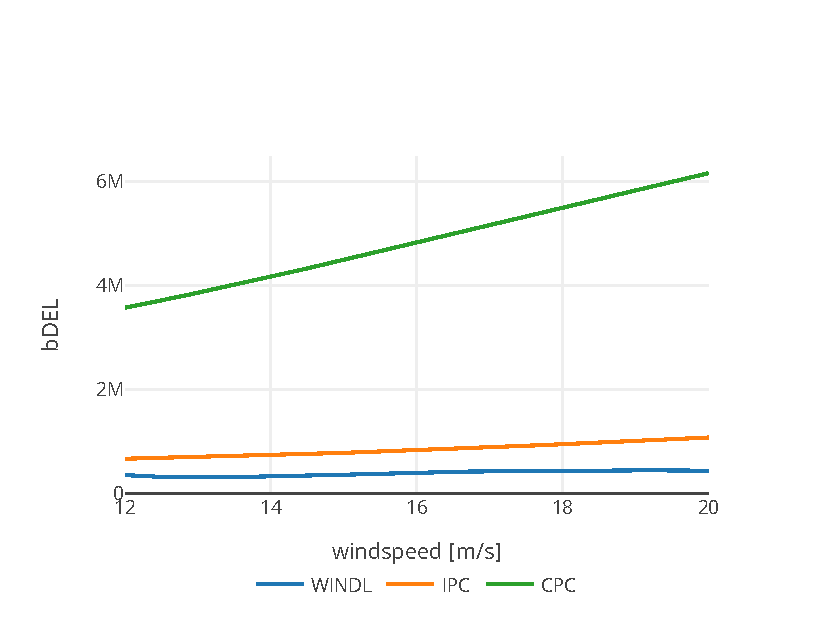
\includegraphics[width=\textwidth]{images/steady_sweep_bdel.pdf}
      \caption{blade-\ac{DEL} against windspeed}
      \label{fig:steady-sweep-bdel}
  \end{subfigure}
  \begin{subfigure}[b]{0.48\textwidth}
      \centering
      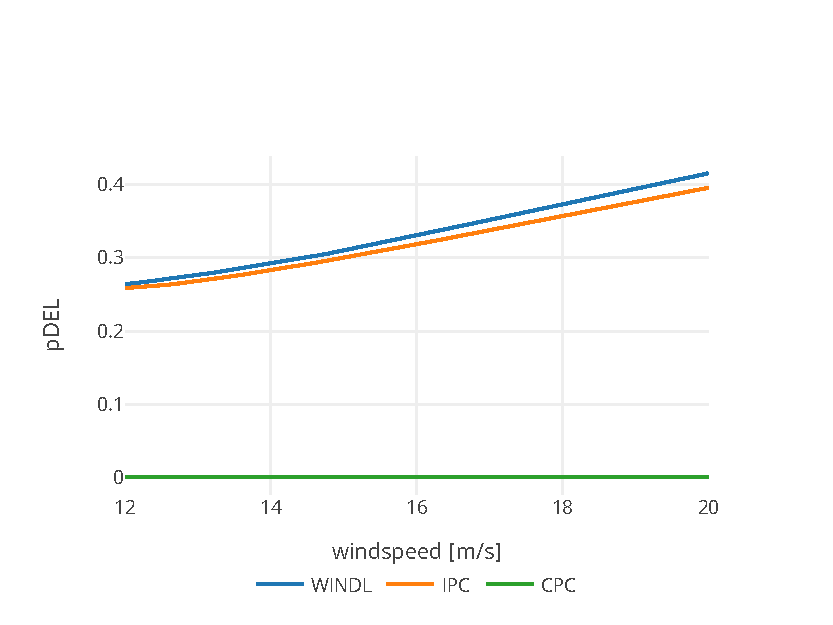
\includegraphics[width=\textwidth]{images/steady_sweep_pdel.pdf}
      \caption{pitch-\ac{DEL} against windspeed}
      \label{fig:steady-sweep-pdel}
  \end{subfigure}
  \caption{bDEL and pDEL metrics for the above-rated operation regime, lower is better. The WINDL controller outperforms both controllers with respect to bDEL, while having a slight hit to pDELs.}
  \label{fig:steady-sweep}
  % sac-steady-final, data_0, reeval_468
\end{figure}

Figure \ref{fig:steady-sweep} shows the evaluation metrics bDEL in \ref{fig:steady-sweep-bdel} and pDEL in \ref{fig:steady-sweep-pdel} for all wind speeds in the above-rated operating regime from 12 to 20 m/s with a resolution of 0.1 m/s, evaluated for the three control policies CPC, IPC, and WINDL. As all control policies and the environment are deterministic, we evaluate a single run for each wind speed. The CPC policy exhibits high bDEL moments but pDEL moments of zero in the steady regime, as it keeps the pitch angles constant. IPC and WINDL both outperform the CPC in terms of DEL moments, as they both employ a policy to account for the wind-shear, but induce pitch actuator wear. The DEL moments induced by WINDL are on average 54.1\% below those of the IPC and 92.0\% below those of the CPC, bringing a significant advantage in blade fatigue wear in comparison to both baselines. This comes at the price of an average of 3.8\% higher pDEL than the IPC.

\subsection{Investigating Policy Actions}

\begin{figure}
  \centering
  \begin{subfigure}[b]{0.48\textwidth}
      \centering
      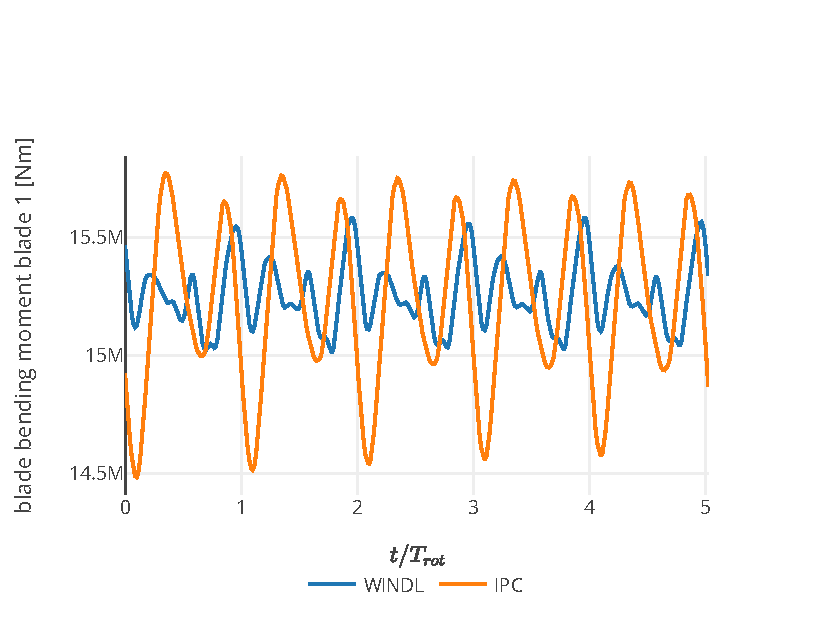
\includegraphics[width=\textwidth]{images/steady_rollout_blade_bending.pdf}
      \caption{Blade bendings against rotor revolutions}
      \label{fig:steady-rollout-blade-bending}
  \end{subfigure}
  \begin{subfigure}[b]{0.48\textwidth}
      \centering
      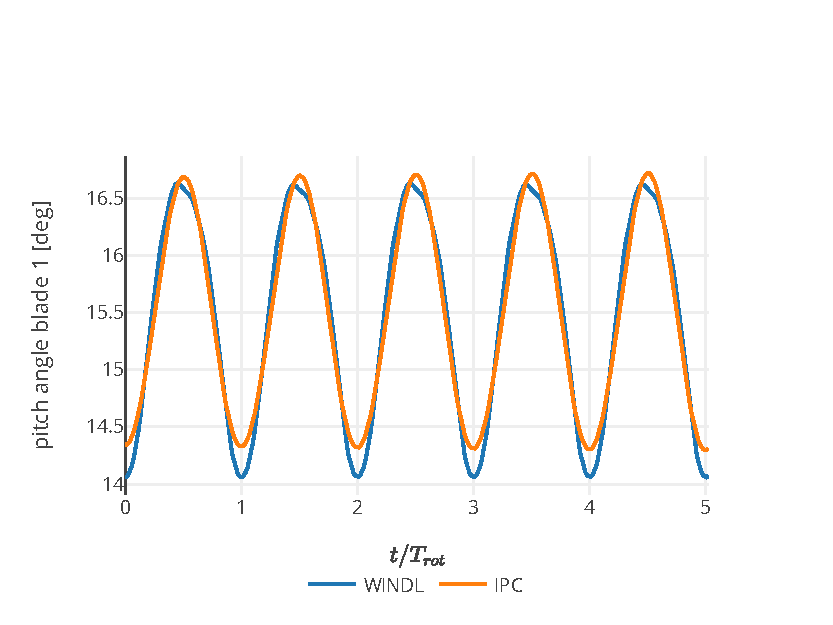
\includegraphics[width=\textwidth]{images/steady_rollout_pitch.pdf}
      \caption{Pitch actuation against rotor revolutions}
      \label{fig:steady-rollout-pitch}
  \end{subfigure}
  \begin{subfigure}[b]{0.48\textwidth}
    \centering
    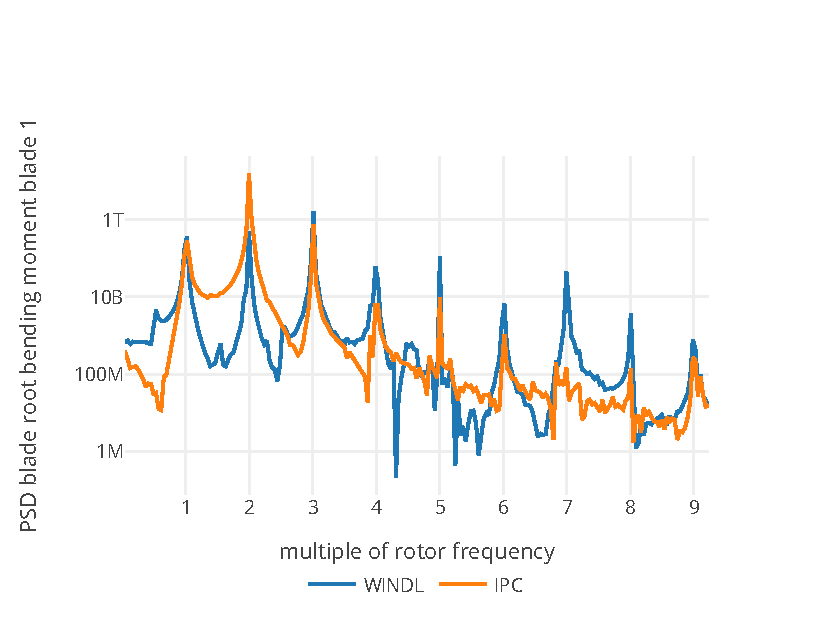
\includegraphics[width=\textwidth]{images/steady_rollout_blade_psd.pdf}
    \caption{Power spectral density plot for blade root bending moments}
    \label{fig:steady-rollout-blade-psd}
  \end{subfigure}
  \begin{subfigure}[b]{0.48\textwidth}
    \centering
    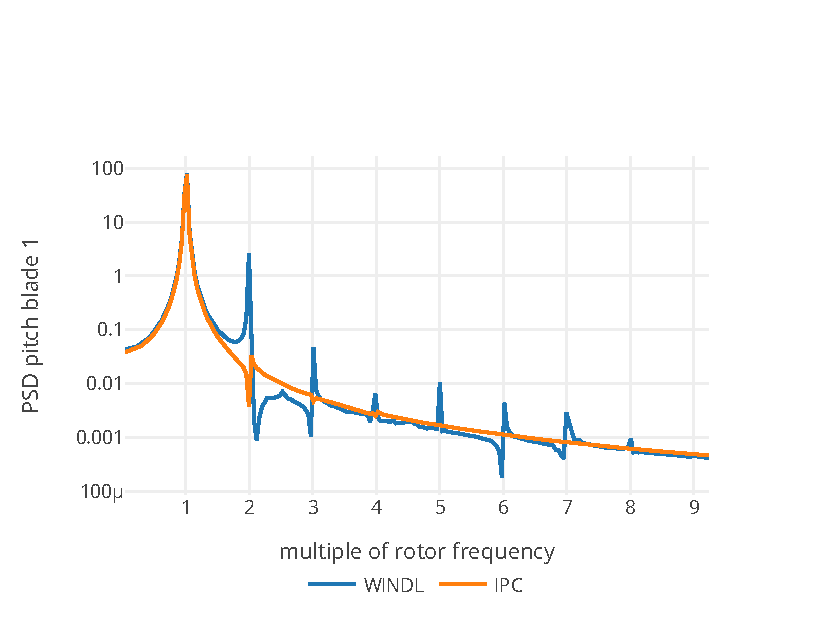
\includegraphics[width=\textwidth]{images/steady_rollout_pitch_psd.pdf}
    \caption{Power spectral density plot for pitch actuation}
    \label{fig:steady-rollout-pitch-psd}
  \end{subfigure}
  \caption{Detailed comparison of WINDL and IPC control policies at a wind speed of 18 m/s. The WINDL policy actuates on a higher number of frequencies, counteracting vibrations on more than the base rotor frequency}
  \label{fig:steady-rollout}
  % sac-steady-final, data_0, reeval_468, run 80 windspeed 18m/s
\end{figure}

To understand how the WINDL controller is able to achieve such a significant improvement, Figure \ref{fig:steady-rollout} compares the WINDL and IPC strategies in detail for a single blade and on a single wind speed of 18 m/s. Bending moments, pitch actuation, and \ac{PSD} for the other two blades are omitted, as they exhibit similar behavior with a delay of a third of a rotation and as such do not provide further information for a qualitative analysis. Other wind speeds are also omitted, as they mainly change the magnitude of pitch actions and blade bendings, not their nature. The wind speed of 18 m/s is chosen as a representative as it most clearly shows the differences between \ac{WINDL} and the IPC baseline. Subplot \ref{fig:steady-rollout-blade-bending} shows the blade root bending moments over rotor revolutions for blade 1. A pattern which repeats every revolution is visible for both policies. Because the inflow conditions are steady, the turbine state is equal every 360 degrees of rotation and a together with a damping control policy, vibrations are constant. Note that we did not explicitely constrain WINDL to have a damping effect, it learned this purely by optimizing the reward function. While the arithmetic mean of the bending moments differ only by 0.1\% between WINDL and IPC, bending moment oscillations induced by the WINDL controller are significantly smaller in amplitude. This smaller amplitude is the driving factor for the bDEL reduction. The relatively small difference in pDELs is caused by a small difference in pitch amplitude, as shown in Subplot \ref{fig:steady-rollout-pitch}. The significant difference between the policies lies in the rich spectral content of the WINDL pitch actuation, as shown in Subplot \ref{fig:steady-rollout-pitch-psd}. While having similar actuation on the 1p frequency, the WINDL controller acts significantly more on the 2p frequency with actuation peaks all the way up to 8p. Especially the effect of the actuation on the 2p frequency shows in the bending moment \ac{PSD}-plot in Subplot \ref{fig:steady-rollout-blade-psd}. At this frequency, WINDL achieves ca. 30 times lower bending oscillation amplitude than the IPC (note the log scale). Even though WINDL exhibits partially higher amplitudes on higher frequencies, this does not offset the saving around 2p.

\subsection{Discussion}

We show WINDL to produce significantly lower fatigue loads than state-of-the-art baseline controllers in the steady wind scenario at the expense of a slight increase in pitch actuation, offsetting the current state-of-the-art by 54.1\%. Instead of trading pDEL for bDEL directly, WINDL actuates with richer spectral contents, achieving a significant bDEL decrease at the cost of just 3.8\% higher pDEL. This shows that WINDL has the potential to match or even outperform state-of-the-art control systems in chosen metrics by black-box optimization only, without requiring information about the underlying physical processes of the environment. 

Albeit the reward function does not incentivize pitch wear reduction ($\rcolemanact=0$), the policy does not trade pitch wear excessively. We attribute this to the smoothness regularization, which smoothes the policy to lower pitch fluctuation. While in theory, further blade wear reductions could be possible by increasing pitch activity on higher frequencies, our pitch actuator model does not support much more activity on high frequencies. Hence, we believe this performance to be close to the optimal performance possible in the steady wind for the given turbine, so WINDL has no reason to increase pitch activity.

The IPC limits its activity to the 1p frequency, whereas WINDL pitches on all frequencies up to 8p. Note that we did not specifically incentivize the rich spectral content; it is purely emerging from black-box optimization given the environment and the reward function. This supports recent findings from traditional wind turbine research, specifically of \citet{vansolingenLinearIndividualPitch2015} which propose a 1p-2p-3p linear pitch controller. In traditional controller design, frequencies above 3p are often disregarded due to the small influence they have on the end result. Also, not every pitch actuator is capable of reproducing such high frequencies. For the IEA-10MW turbine, the 1p rotation frequency corresponds to 0.14 Hz, hence 8p would be at around 1.15 Hz. Oscillating the massive 48 ton blades at this frequency is at the limits of physically possible. However, for the simplistic actuator model used in this work, it seems to play out favorably to pitch on such high frequencies. These experiments show that black-box optimization through WINDL can be used to reinforce and improve scientific understanding in the field of wind turbine control.

Depending on the turbine and operating site, the \ac{LCOE} can benefit differently from component load relief. A turbine model can have sensitive blades and require the maximum possible blade wear relief, or be more sensitive to pitch wear. Currently, the IPC policy is commonly used on turbines that benefit from blade load reductions past the capabilities of a CPC. With our findings, we show that the \ac{WINDL} policy could be a good fit for such situations as well, providing further blade load relief than the IPC policy. Our strategy extends the range of options for wind turbine manufacturers and operators to choose the best possible strategy for their turbine.

\section{Transition Around Rated Wind Speed}
\label{section:results-transition}

\begin{summary}
In this section, we demonstrate that WINDL produces lower fatigue loads at the cost of power around rated speed in the steady wind scenario. We measure blade fatigue loads and power production around rated speed and then follow up with two rollouts. Along with the rollouts, we investigate a phenomenon where WINDL utilizes the individual blades very unevenly below rated speed.
\end{summary}

For this section, we evaluate the same model as in Section \ref{section:results-steady-fatigue} in wind speeds between 10 and 12 m/s around the rated wind speed of the turbine.

The transition period around rated speed poses significant challenges in wind turbine control due to two major reasons, high thrust and controller design. The aerodynamic thrust on the rotor is at its maximum at rated (see Figure \ref{fig:IEA10MW}), as the regulation of the pitch controller above rated speed decreases rotor thrust faster than the increase in wind speed can increase thrust. Hence, the turbine is especially susceptible to extreme loads in this operating range. Furthermore, controller design theory works with a switch in control systems at rated speed. Below rated, the torque controller regulates the turbine, and above the pitch controller does. This leaves the question open to what happens \textit{at} rated speed, and current methods mainly focus on getting the policy switch to work without having a specific optimization criterium in mind \cite[Section 8.3.4]{burtonWindEnergyHandbook2011}. 

\subsection{Presentation}

\begin{figure}
  \centering
  \begin{subfigure}[b]{0.48\textwidth}
      \centering
      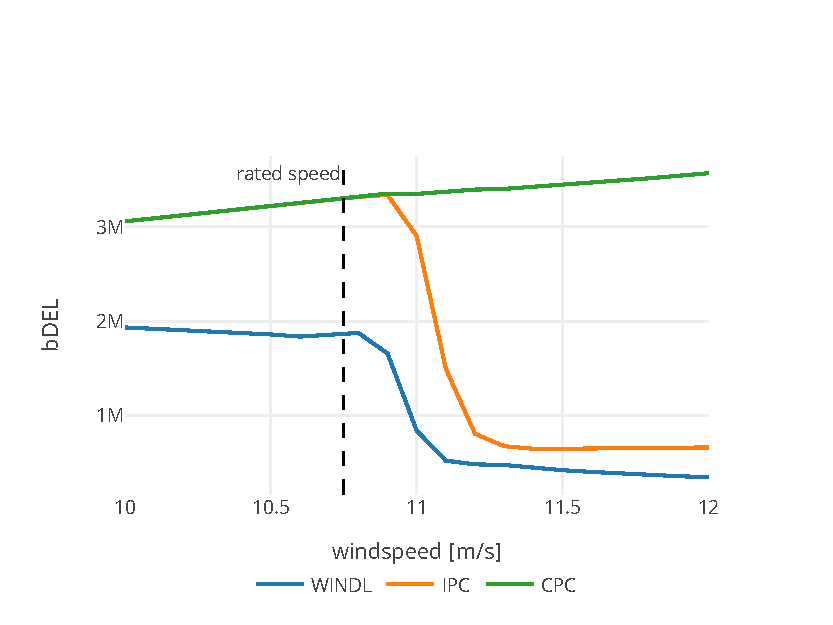
\includegraphics[width=\textwidth]{images/transition_bdel.pdf}
      \caption{Blade-\ac{DEL} against windspeed}
      \label{fig:transition-bdel}
  \end{subfigure}
  \begin{subfigure}[b]{0.48\textwidth}
      \centering
      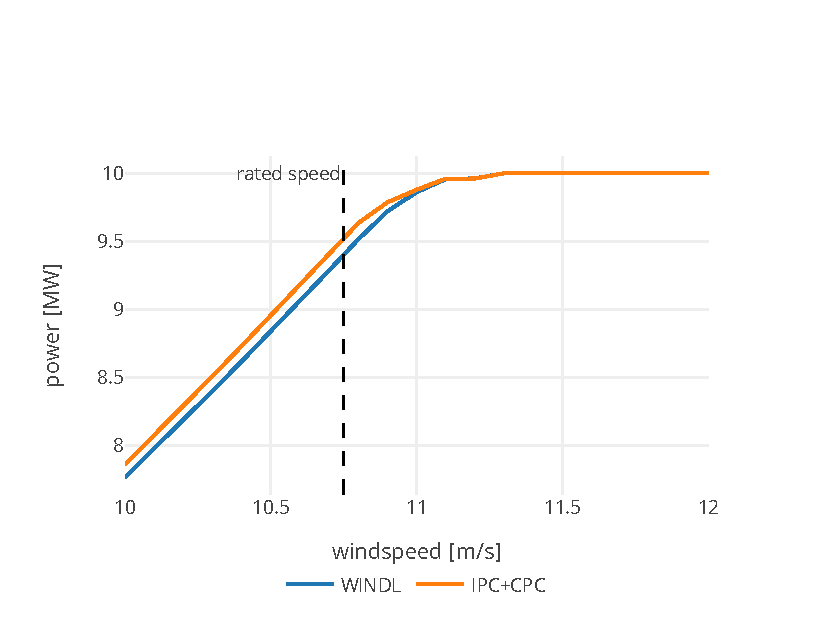
\includegraphics[width=\textwidth]{images/transition_power.pdf}
      \caption{Average power production against windspeed}
      \label{fig:transition-power}
  \end{subfigure}
  \caption{Blade-DEL and power production against windspeed in the transition period around rated speed. WINDL offers significantly lower blade DELs at the cost of some power loss.}
  \label{fig:transition}
  % sac-steady-final, data_0, reeval_468 
\end{figure}

Figure \ref{fig:transition} shows the bDEL metric and average power production for CPC, IPC, and WINDL control policies. The rated speed of the IEA-10MW turbine is indicated by a dashed line at 10.75 m/s. In \ref{fig:transition-power}, the power curve of CPC and IPC are exactly equal. This is due to the IPC being designed such that it ramps down its activity at slightly above rated speed before any power is lost \cite{perez-beckerImplementationValidationAdvanced2021}. For the IEA-10MW turbine, the ramp-down is scheduled between 11.2 and 10.9 m/s, as visible in the IPC curve in \ref{fig:transition-bdel}. WINDL exhibits a power reduction of 1.23\% at rated speed, or 0.62\% reduction averaged across the shown transition period of 10 m/s to 12 m/s. In turn, it achieves a bDEL reduction of 42.9\% compared to the IPC baseline, and 64.1\% compared to the CPC baseline across the transition period. 

Both WINDL and the IPC experience a sharp increase in bDEL for small decreases in wind speed around 11 m/s. For WINDL, bDELs jump up from 0.42M at 11.5 m/s to 1.71M at rated speed, for the IPC they jump from 0.65M at 11.5 m/s to 3.3M at rated speed. Such a sharp increase is the result of two phenomena occurring in parallel, maximal rotor thrust and minimal pitch activity. For the IPC, this is exacerbated by the activity ramp-down, which transitions into a CPC policy at rated. For WINDL, the sinusoidal motion, which is possible above rated, is cut off below rated due to the cap in pitch angle at 0 degrees. This introduces the need for a different policy at rated speed. 

\subsection{Different Blade Action Phenomenon At Rated Speed}

\begin{figure}
  \centering
  \begin{subfigure}[b]{0.48\textwidth}
      \centering
      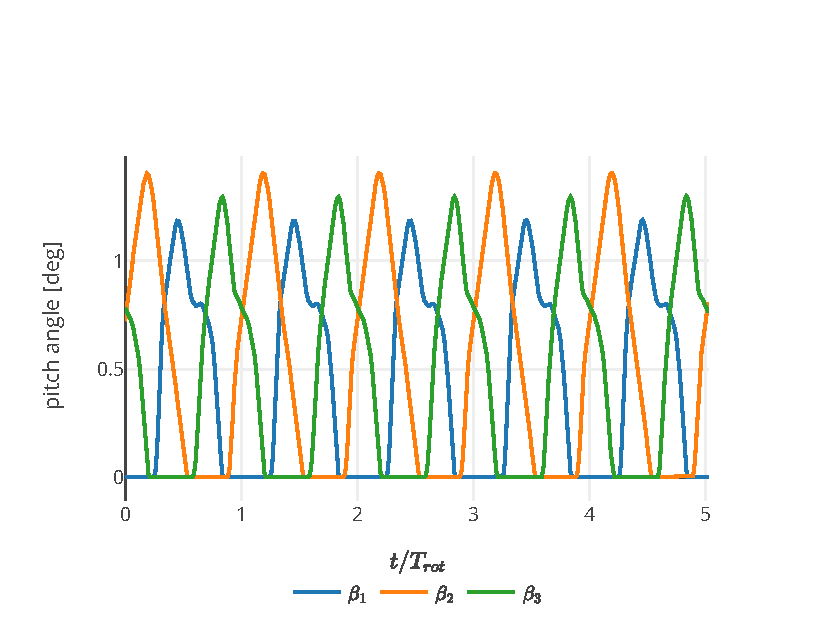
\includegraphics[width=\textwidth]{images/pitch_angle_rollout_10_7ms.pdf}
      \caption{WINDL pitch activity at 10.7 m/s (rated speed)}
      \label{fig:pitch-at-rated}
      % run 7
  \end{subfigure}
  \begin{subfigure}[b]{0.48\textwidth}
      \centering
      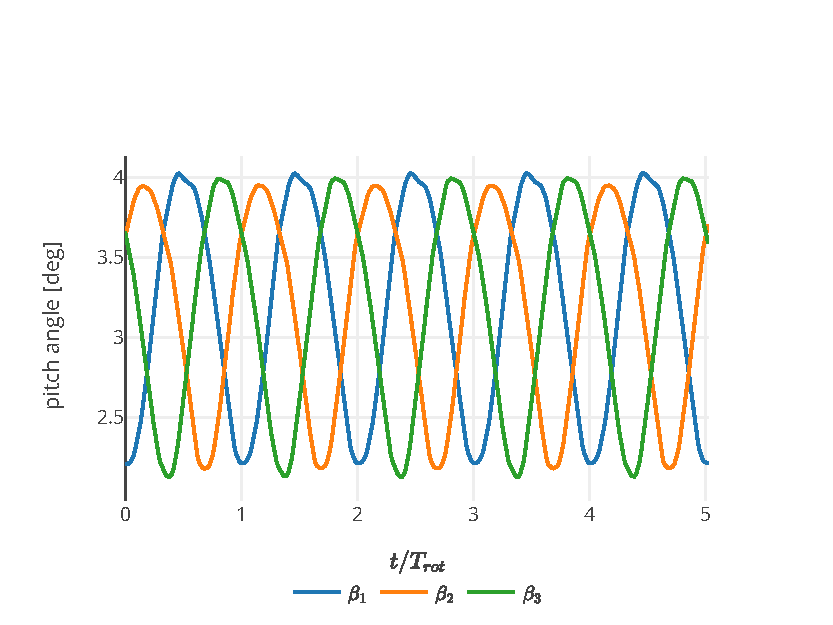
\includegraphics[width=\textwidth]{images/pitch_angle_rollout_11_5ms.pdf}
      \caption{WINDL pitch activity at 11.5 m/s}
      \label{fig:pitch-above-rated}
      % run 15
  \end{subfigure}
  \caption{WINDL pitch activity at rated and slightly above rated speed. While above rated speed, the pitching motion is sinusodial, it is capped and asymmetric at rated speed.}
  \label{fig:pitch-around-rated}
  % sac-steady-final, data_0, reeval_468
\end{figure}

Figure \ref{fig:pitch-around-rated} shows the different pitch behavior of \ac{WINDL} at and above rated speed. Slightly above rated speed, a symmetrical sinusoidal motion is applied to all blades similar to Figure \ref{fig:steady-rollout-pitch}. At rated speed, this motion is cut off at 0 degrees. In Subfigure \ref{fig:pitch-at-rated}, a phenomenon can be observed where the different blades are actuated visibly differently. Blade number two performs a high-magnitude and close to sinusoidal motion, while blade one and three are actuated with a lower magnitude. The bDEL values for the individual blades at 10.7 m/s are $[1.88\text{M}, 1.51\text{M}, 1.73\text{M}]$. There is no explicit incentive to actuate evenly across all blades, but for higher wind speeds like in Subfigure \ref{fig:pitch-above-rated} the policy intrinsically keeps their motions similar. Note that even in this plot, there is a slight difference in actuation rate. We hypothesize the uneven behavior at rated speed to be optimal or at least not penalized in the reward function. Keeping a full sinusoidal motion for every blade is impossible due to the low base pitch angle. To keep one blade as close to a sinusoidal motion as possible (blade 2 in this case) and to use the other two to keep up the thrust might improve the total reward more than having all three incur equally bad loads. We briefly investigated a reward penalty for differing behavior of the individual blades but found this to not solve the problem.

\subsection{Discussion}

We show WINDL to produce significantly lower bDELs in the transition period from 10 to 12 m/s, offsetting the current state-of-the-art by 42.9\%. This comes at the expense of a decrease in power of 0.62\%. We see a peak in loads at rated speed, which is consistent with expectations for all policies. Using a load-minimizing policy that can work at rated speed brings high load saving potential. While above rated, WINDL does not exhibit a decrease in power, some power yield is lost in the transition period. For most wind turbine models, such a significant impact on the total energy yield of the wind turbine likely offsets the benefit of lower blade loads by a wide margin. To judge whether the decrease in power is justified by the load reduction, an extensive analysis is required, taking into account material properties, electricity sale prices, and the weather on site. The result of this analysis would be a wind speed threshold, below which it is not feasible to operate WINDL anymore and where it should be ramped down. Technically, it could be operated all the way down to set-in speed, but we only expect an application below rated wind speed to be sensible in very few situations.

Furthermore, we observe a phenomenon around rated speed, where WINDL exhibits unequal pitching action. Our current reward function might incentivize this behavior and we found no trivial way to disincentivize it. It could even be globally optimal to do so, as the higher load on the two other blades might be overcompensated by the lower load on blade number two. To evenly distribute wear, a fix could involve rotating the pitch action mappings to the blades, so each blade gets to be number two at some point. Future work could try to investigate this phenomenon or find a better fix.

\section{Naive Performance Turbulent Wind}
\label{section:results-naive-turbulent}

\begin{summary}
In this section, we train WINDL in the turbulent wind using the same hyperparameters as used for the steady wind. We find that this results in slightly better blade wear but brings a disproportionate hit to pitch wear and power yield. We conclude that different hyperparameters are needed for different wind scenarios.
\end{summary}

For this section, we train a model with four different random seeds in the turbulent wind scenario to 1000 epochs (16M environment interactions) and choose the best performing checkpoint with respect to bDEL. We use the same hyperparameters as in the steady wind, see Table \ref{table:hyperparameters}. For our evaluation, we measure performance on all wind speeds between 10 and 20 m/s across eight random seeds and with a resolution of 0.1 m/s steps.

Depending on the location of a turbine, it will not only experience steady wind during operation. Thunderstorms, strong thermal convection, or other phenomena can cause the wind to rapidly change speed and direction. Such a rapid change can cause structural damage through high loads on a wind turbine, if the load minimizing control policy is not able to counteract in time. While in the steady wind, the major trade-off concerns only blade and pitch wear, in the turbulent wind there is a three-way trade-off between power yield, blade wear, and pitch wear. A good control policy pitches aggressively at the start of strong gusts to reduce blade wear and pitches conservatively in low winds to maximize energy yield. It optimizes power yield, blade fatigue loads, blade extreme loads, and pitch fatigue loads simultaneously. Optimally, WINDL can learn this with the same hyperparameters that yielded good results in the steady wind scenario showing hyperparameter insensitivity.

\subsection{Presentation}

\begin{figure}[hbt!]
  \centering
  \begin{subfigure}[b]{0.48\textwidth}
      \centering
      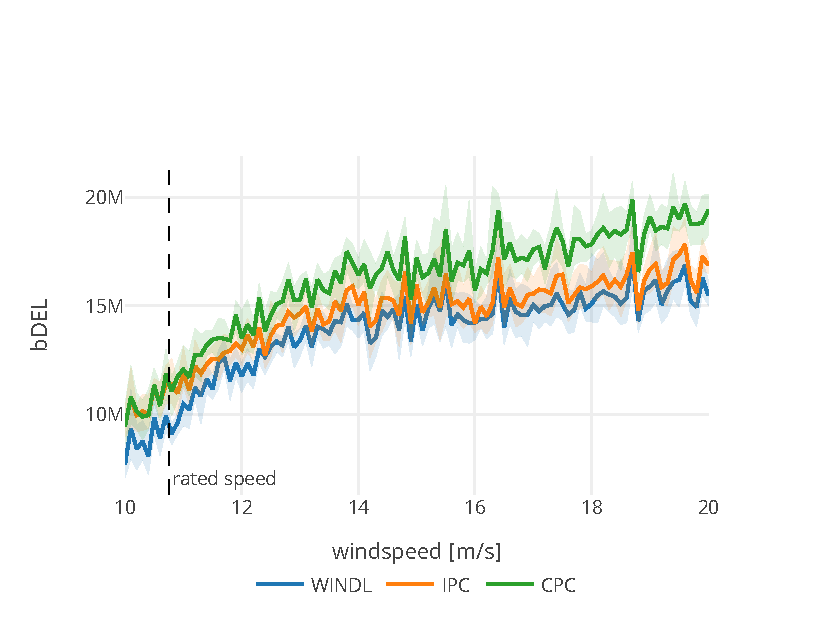
\includegraphics[width=\textwidth]{images/naive_sweep_bdel.pdf}
      \caption{blade-DELs against windspeed}
      \label{fig:naive-sweep-bdel}
  \end{subfigure}
  \begin{subfigure}[b]{0.48\textwidth}
      \centering
      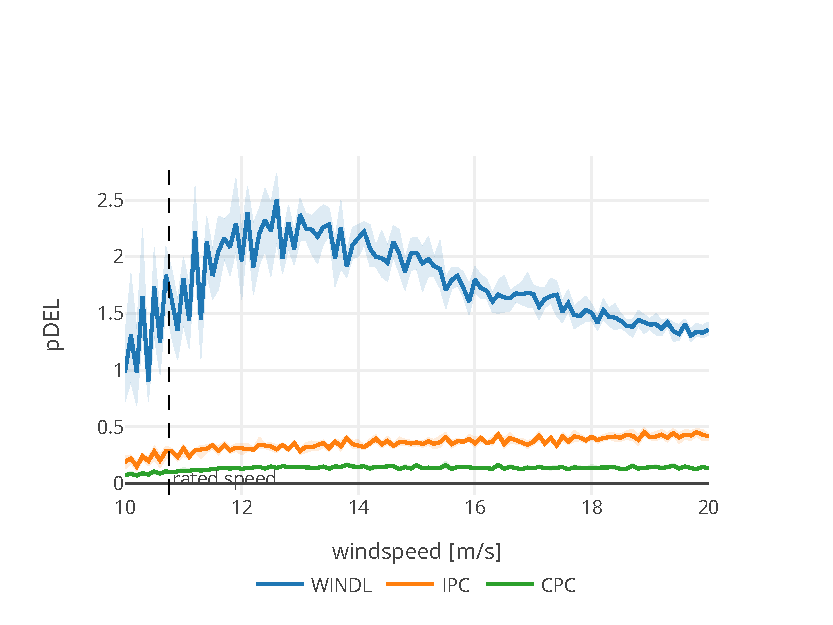
\includegraphics[width=\textwidth]{images/naive_sweep_pdel.pdf}
      \caption{pitch-DELs against windspeed}
      \label{fig:naive-sweep-pdel}
  \end{subfigure}
  \begin{subfigure}[b]{0.48\textwidth}
    \centering
    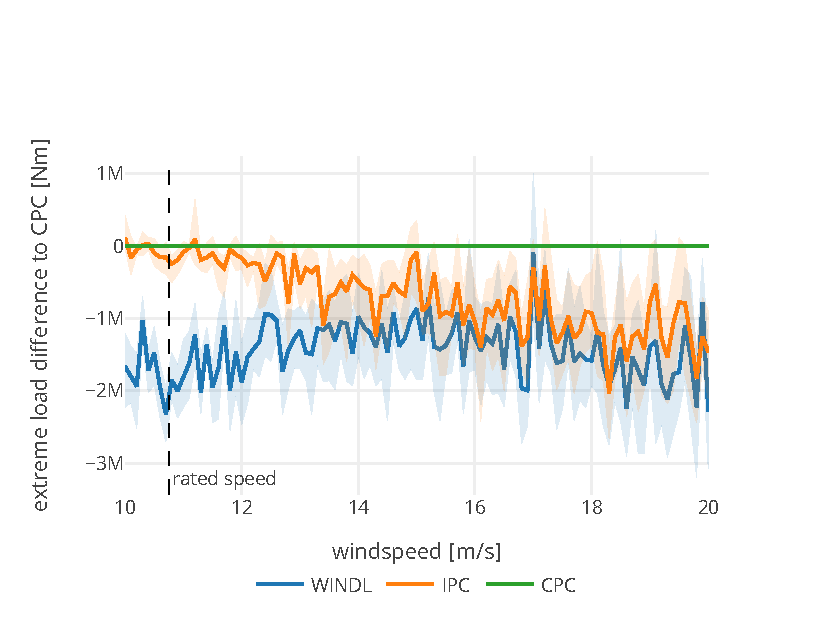
\includegraphics[width=\textwidth]{images/naive_sweep_extreme.pdf}
    \caption{Relative extreme loads compared to CPC performance against windspeed}
    \label{fig:naive-sweep-extreme}
\end{subfigure}
\begin{subfigure}[b]{0.48\textwidth}
    \centering
    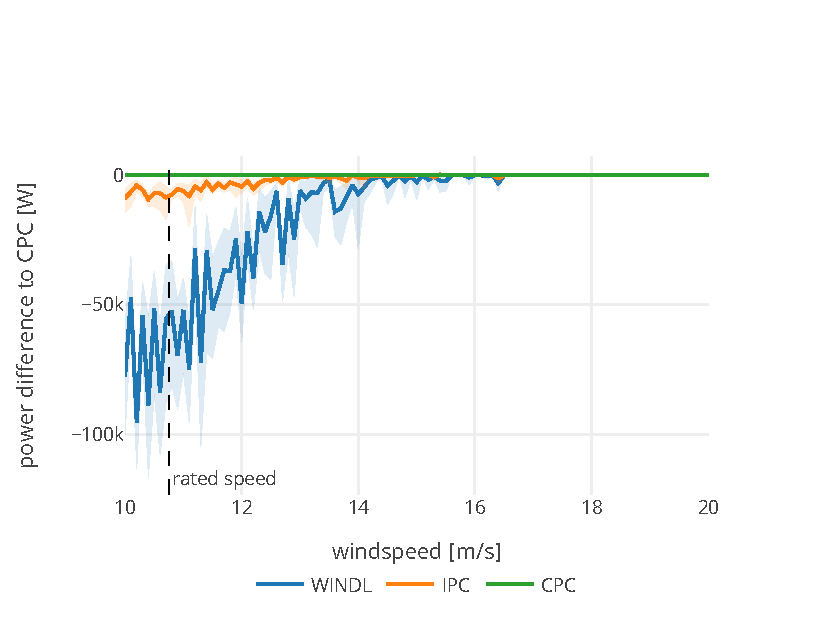
\includegraphics[width=\textwidth]{images/naive_sweep_power.pdf}
    \caption{Relative power production compared to CPC performance against windspeed}
    \label{fig:naive-sweep-power}
\end{subfigure}
  \caption{The transfer performance of a model trained in the turbulent wind scenario with hyperparameters from the steady wind, compared to IPC and CPC performance. Lower is better except for power production.}
  \label{fig:naive-sweep}
  % sac-fullturb-5, data_12, reeval_225
\end{figure}

\begin{table}[hbt!]
  \centering
  \begin{tabular}{c@{\hskip 0.7cm}cc@{\hskip 0.7cm}cc}
    \toprule
    & \multicolumn{2}{c}{WINDL to IPC} & \multicolumn{2}{c}{WINDL to CPC} \\
    Metric & 10-12 m/s & 12-20 m/s & 10-12 m/s & 12-20 m/s \\
    \midrule
    bDEL & -1.26M (11.19\%) & -0.74M (4.61\%) & -1.69M (13.94\%) & -2.47M (14.11\%) \\
    pDEL & +1.40 (-532\%) & +1.41 (-403\%) & +1.56 (-1402\%) & +1.64 (-1180\%) \\
    extreme [Nm] & -1.60M (4.62\%) & -0.55M (1.85\%) & -1.71M (4.91\%) & -1.37M (4.78\%) \\
    power [W] & -50.3K (-0.58\%) & -3.80K (-0.04\%) & -56K (-0.65\%) & -4.27K (-0.04\%) \\
    \bottomrule
  \end{tabular}
  % sac-fullturb-4, data_12, reeval_225
  \caption{Mean absolute difference and mean relative improvement of naive WINDL as shown in Figure \ref{fig:naive-sweep} compared to the IPC and the CPC, split in around-rated (10-12 m/s) and above-rated (12-20 m/s).}
  \label{table:naive-improvements}
\end{table}

Figure \ref{fig:naive-sweep} shows the performance of a WINDL policy that was chosen among four trainings to 1000 epochs by picking maximal bDEL performance. Four different metrics are evaluated for different wind speeds in the range of 10 to 20 m/s across eight turbulent seeds per wind speed with a wind speed resolution of 0.1 m/s. Subplot \ref{fig:naive-sweep-bdel} and Subplot \ref{fig:naive-sweep-pdel} plot absolute values, while Subplot \ref{fig:naive-sweep-extreme} and Subplot \ref{fig:naive-sweep-power} plot relative values to CPC performance to improve readability of the plots. The averaged absolute differences to the baselines, and in brackets the averaged relative improvements of these performances, are shown in Table \ref{table:naive-improvements}. Note that for bDEL, pDEL and extreme loads, less is better, while for power, more is better.

WINDL exhibits lower blade fatigue loads than the IPC baseline by 4.61\% above rated and 11.19\% around rated (Subplot \ref{fig:naive-sweep-bdel}). An improvement can be seen across the entire range of wind speeds, but most prominently up to 14 m/s. Also, WINDL exhibits lower extreme loads as visible in Subplot \ref{fig:naive-sweep-extreme}. Between 10 and 12 m/s, extreme loads are 4.65\% lower than the IPC baseline and 4.95\% lower than the CPC, while above rated between 12 and 20 m/s, they are 1.91\% lower than the IPC and 4.68\% lower than the CPC. This comes at the price of significantly higher pitch DELs by 376\% compared to the IPC and 1157\% compared to the CPC (Subplot \ref{fig:naive-sweep-pdel}). Also, WINDL exhibits power losses of 3.8 kW compared to the IPC above rated and 50 kw below rated (Subplot \ref{fig:naive-sweep-power}). The power loss is only significantly visible below 14 m/s and not visible anymore above 16.5 m/s.  Because above 16.5 m/s wind speed, most turbulences in the \ac{NTM} do not reach speeds below rated, the generator stays at saturation levels the entire time.

Compared to the policy performance in Figure \ref{fig:transfer-turbulent}, the blade DELs are better. The pitch wear exhibited by the policy trained in the turbulent wind is worse than the policy trained in the steady wind but evaluated in turbulent. In contrast to the steady wind in Figure \ref{fig:transition}, blade and pitch wear do not peak at rated speed for any of the control policies. The absence of this peak is caused by the magnitude of wear induced through turbulence, which overshadows wear induced by control policies. When compared to the steady wind above rated performance in Figure \ref{fig:steady-sweep}, both blade and pitch wear values are higher by ca. one order of magnitude. As such, wear effects induced by the steady wind shear and control policies are overshadowed by the wear induced through turbulences.

\subsection{Discussion}

WINDL outperforms the IPC with respect to blade DELs by 4.6\% above rated. 

Besides reducing blade fatigue loads in the DEL metric, WINDL does also reduce extreme loads below IPC levels. There is an incentive to do so, because the reward function will react negatively to extreme loads. As extreme loads are relatively short events, the high-pass filter for the $\tilde c_s$ component will not filter them out, and they will increase the blade penalty. Especially at rated speed where extreme loads are high, this significant decrease can prevent fatal damage to blades in gusts. Furthermore, blades can be designed with a lower breaking point, which will reduce construction costs.

Section \ref{section:results-steady-fatigue} has shown WINDL to be capable of finding a high performing policy for the steady wind scenario with regards to both optimization aims from the steady wind: pitch wear and blade wear. While in the steady wind, it is not explicitly incentivized to keep pitch activity low, the smoothness regularization automatically does so. In the turbulent scenario, this is not the case. The agent trained on the turbulent wind learns to pitch more aggressively than an agent trained on the steady wind, which shows that the agent exploits the pitch blade trade-off to optimize blade bendings only. This exploitation is a major argument against WINDL adoption, and pitch wear of that magnitude is likely not acceptable even for turbines with sturdy pitch bearings. 

The exploitation does also apply to power production, and as soon as WINDL has the option to trade it for blade bending, it does so. Power production is not captured at all by our reward function. While the assistive CPC has the aim to maximize power, the reinforcement learned load control policy manages to interfere with this policy.

Concludingly, WINDL does successfully optimize the primary optimization goal blade wear below IPC levels. However, the naive policy is not well suited as a drop-in replacement for IPC controllers, because it disregards secondary optimization aims. While in the steady wind, an explicit penalty for pitch wear is not necessary, the turbulent wind scenario requires a hyperparameter modification to regard secondary optimization aims.

\section{Adjusted For Pitch Loads}
\label{section:results-adjusted}

\begin{summary}
In this section, we train WINDL with an adjusted hyperparameter set in the turbulent wind. We find that the adjusted WINDL produces significantly lower blade loads than current baseline controllers, potentially setting a new state-of-the-art for wind turbine load control. However, we observe drawbacks through more pitch wear and some power loss. We investigate two example rollouts to observe the strategies that WINDL learned and find that it can choose when to utilize pitch actions smartly and that it pitches through low-wind scenarios to alleviate extreme loads.
\end{summary}

To train the model for this section, we utilize adjusted hyperparameters for the turbulent wind, as outlined in the rightmost column of Table \ref{table:hyperparameters}. These hyperparameters were obtained by tuning for both blade and pitch wear. We train four random seeds up to 1500 epochs, which corresponds to 36M environment interactions, and pick the best performing checkpoint with respect to bDEL for evaluation.

Reinforcement learning algorithms are benchmarked on a variety of tasks and shall perform well on all of them without changes to hyperparameters. In our case, we can tune the hyperparameters to the specific task at hand to reach maximal performance. For a production use of WINDL, one hyperparameter set for all wind scenarios would be desirable, but for a proof of concept, different sets can show the potential performance gains. 

To obtain these results, we perform a hyperparameter search with the aim of finding the best set of hyperparameters for the turbulent wind. Best referrs mainly to final policy performance, with training stability and convergence speed as secondary aims. The new set of hyperparameters is presented in Table \ref{table:hyperparameters} in the column \textit{turbulent wind}. Smoothing parameters were increased to $\lambdatemp=0.2, \lambdaspat=0.2$, but in contrast to the steady wind, purely smoothness regularized pitch control exhibited too high pitch activity. The pitch performance did not differ much from naive performance as shown in Section \ref{section:results-naive-turbulent}. Adding the pitch penalty $\rcolemanact=0.02$ into the reward function improved pitch handling, but significantly destabilized training. Decreasing the learning rates by factor 3, increasing the discounting factor to $\gamma=0.99$, and increasing the number of environment interactions per epoch by 50\% alleviated these issues. Lastly, slightly increasing IPC control play to $\ipcplay=\pm4$ and allowing $c_S$ action control drastically improved blade wear with just a marginal hit to pitch activity.

\subsection{Presentation}

\begin{figure}[hbt!]
  \centering
  \begin{subfigure}[b]{0.48\textwidth}
      \centering
      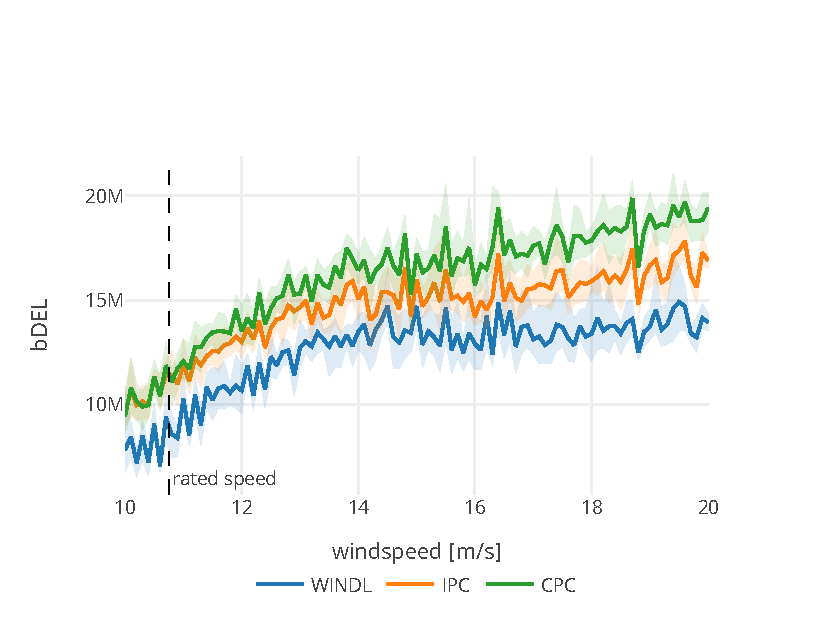
\includegraphics[width=\textwidth]{images/adjusted_bdelopt_bdel.pdf}
      \caption{blade-DELs against windspeed}
      \label{fig:adjusted-bdelopt-bdel}
  \end{subfigure}
  \begin{subfigure}[b]{0.48\textwidth}
      \centering
      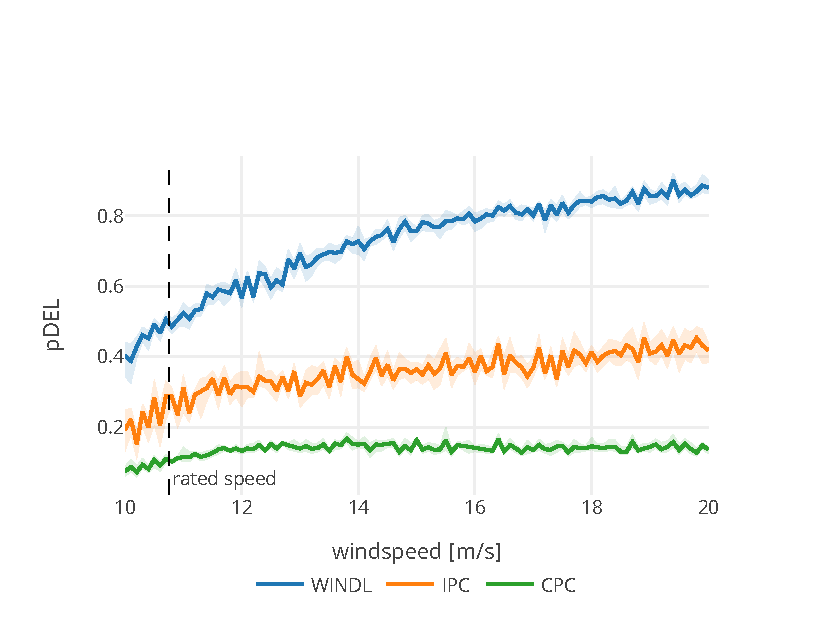
\includegraphics[width=\textwidth]{images/adjusted_bdelopt_pdel.pdf}
      \caption{pitch-DELs against windspeed}
      \label{fig:adjusted-bdelopt-pdel}
  \end{subfigure}
  \begin{subfigure}[b]{0.48\textwidth}
    \centering
    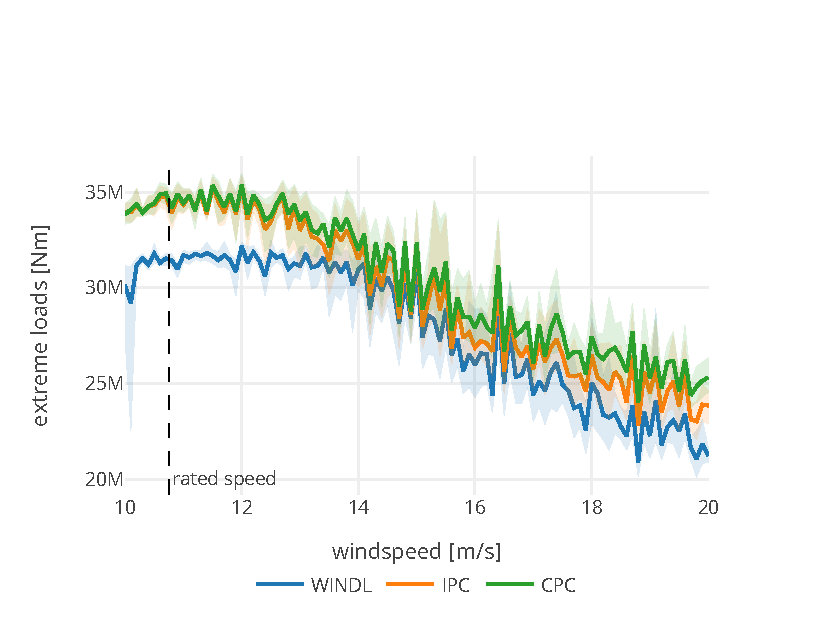
\includegraphics[width=\textwidth]{images/adjusted_bdelopt_extreme.pdf}
    \caption{Extreme loads against windspeed}
    \label{fig:adjusted-bdelopt-extreme}
  \end{subfigure}
  \begin{subfigure}[b]{0.48\textwidth}
      \centering
      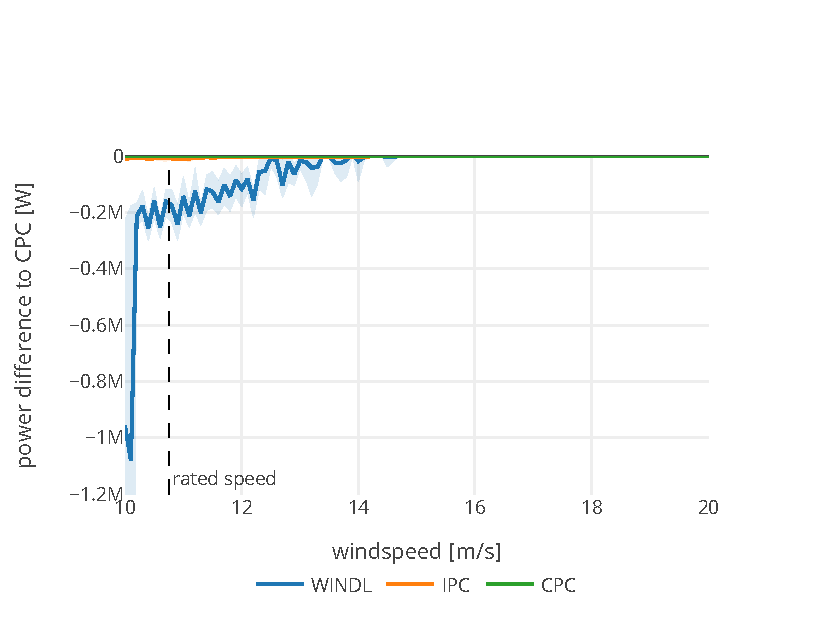
\includegraphics[width=\textwidth]{images/adjusted_bdelopt_power.pdf}
      \caption{Relative power production compared to CPC performance against windspeed}
      \label{fig:adjusted-bdelopt-power}
  \end{subfigure}
  \caption{The performance of adjusted WINDL, compared to IPC and CPC performance. Lower is better except for power production.}
  \label{fig:adjusted-bdelopt}
  % sac-turb-optim-1, data_42, turb_reeval_1430
\end{figure}

\begin{table}[hbt!]
  \centering
  \begin{tabular}{c@{\hskip 0.7cm}cc@{\hskip 0.7cm}cc}
    \toprule
    & \multicolumn{2}{c}{WINDL to IPC} & \multicolumn{2}{c}{WINDL to CPC} \\
    Metric & 10-12 m/s & 12-20 m/s & 10-12 m/s & 12-20 m/s \\
    \midrule
    bDEL & -2.27M (19.8\%) & -2.11M (13.45\%) & -2.69M (22.28\%) & -3.85M (22.04\%) \\
    pDEL & +0.24 (-111\%) & +0.4 (-110\%) & +0.4 (-386\%) & +0.63 (-455\%) \\
    extreme [Nm] & -3.07M (8.86\%) & -1.56M (5.45\%) & -3.17M (9.14\%) & -2.39M (8.27\%) \\
    power [W] & -241K (-2.83\%) & -9.38K (-0.1\%) & -247K (-2.89\%) & -9.77K (-0.1\%) \\
    \bottomrule
  \end{tabular}
  % sac-turb-optim-1, data_42, turb_reeval_1430
  \caption{Mean absolute difference and mean relative improvement of adjusted WINDL compared to the IPC and the CPC, split in around-rated (10-12 m/s) and above-rated (12-20 m/s).}
  \label{table:improvements-bdelopt}
\end{table}

Figure \ref{fig:adjusted-bdelopt} and Table \ref{table:improvements-bdelopt} show the final policy performance of a policy trained with the adjusted hyperparameters for the turbulent wind. The performance of the WINDL, IPC and CPC policy is evaluated in eight different turbulent seeds for all wind speeds from 10 - 20 m/s with a resolution of 0.1 m/s. All subplots in Figure \ref{fig:adjusted-bdelopt} show absolute values except for Subplot \ref{fig:adjusted-bdelopt-power}, which shows relative values compared to the CPC policy to improve readability.

Across the entire wind span, a significant reduction in bDELs compared to the difference between IPC and CPC is visible (Subplot \ref{fig:adjusted-bdelopt-bdel}). The first row in Table \ref{table:improvements-bdelopt} quantifies this to 13\% lower blade wear above rated compared to the current state-of-the-art. Especially around rated speed, where the IPC does not improve upon the CPC a lot, WINDL still delivers a significant fatigue load reduction. 

This comes at the price of higher blade DELs as visible in Subplot \ref{fig:adjusted-bdelopt-pdel}. Pitch actuation rises with wind speed and relative wear levels are consistent to approximately double the IPC rates across the entire operating range (row 2, Table \ref{table:improvements-bdelopt}). 

The IPC is deactivated in around- and below-rated wind speeds to prevent power loss, which results in only a 0.015\% decrease from CPC to IPC. WINDL exhibits one order of magnitude higher power losses above rated (-0.1\%) and two orders of magnitude higher around rated speed (-2.89\%) compared to the CPC, which generates the maximum amount of power (see row 4, Table \ref{table:improvements-bdelopt}). As visible in Subplot \ref{fig:adjusted-bdelopt-power}, this loss happens mostly below 14 m/s, and above 16 m/s no more power losses are measurable. Congruent to previous policies, this is consistent with the turbulence model, which will not dip below rated speed for mean wind speeds above 16 m/s.

Together with the loss in power, the reduction of extreme loads is most prominent below 14 m/s (see Subplot \ref{fig:adjusted-bdelopt-extreme}). Around rated, an extreme load reduction of 8.86\% compared to the IPC policy is achieved (see row 3 Table \ref{table:improvements-bdelopt}). This extreme load reduction coincides with the power loss and might be due to WINDL exploiting a trade-off. Around rated, extreme values are maximal and an extreme load reduction is most desired. The highest extreme load across all seeds is reduced from 3.9M Nm for the IPC to 3.5M Nm for WINDL with mean values well below that (see lower wind speeds in Subplot \ref{fig:adjusted-bdelopt-extreme}). Above rated, an improvement of 5.45\% compared to the IPC is visible. Some of this improvement is to be credited to the loss in power, which allows for an extreme load saving policy around rated speed. Taking into account only the region from 14 m/s to 20 m/s where WINDL does not lose much power, the improvement drops to 5.3\%.

Compared to the naive policy as presented in Section \ref{section:results-naive-turbulent}, the hyperparameter adjustments have brought a significant improvement in all quantities subject to optimization except for power. When directly comparing Table \ref{table:improvements-bdelopt} to Table \ref{table:naive-improvements}, the adjusted WINDL achieves significantly lower blade bendings, pitch bendings, and extreme load than the naive version.

\subsection{Investigating Policy Actions}

In this subsection, we pick two example rollouts in different wind scenarios to clarify the difference between the WINDL and IPC policy. We demonstrate how WINDL gains upon the IPC and investigate the power loss phenomenon.

\begin{figure}[hbt]
  \centering
  \begin{subfigure}[b]{0.48\textwidth}
      \centering
      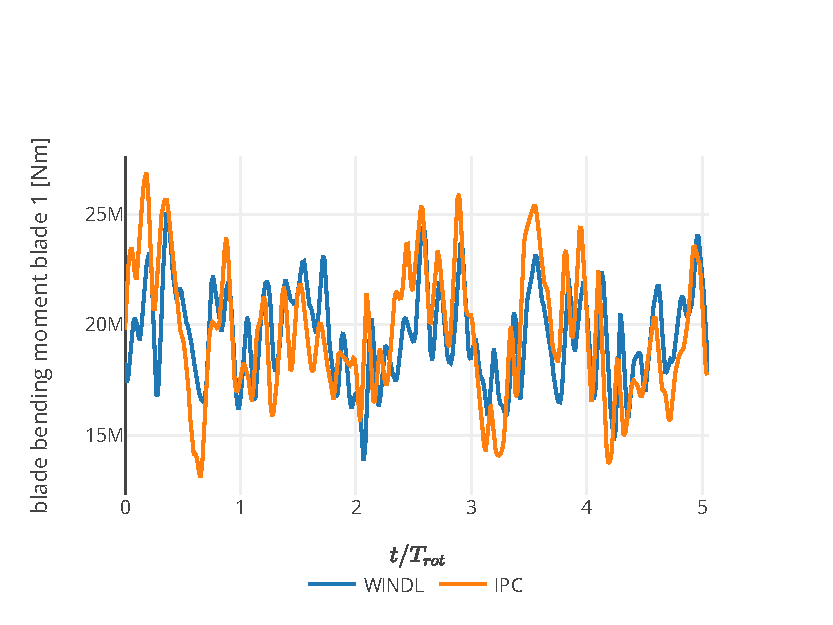
\includegraphics[width=\textwidth]{images/adjusted_blade_rollout.pdf}
      \caption{Blade bendings over time for mean wind speed 14 m/s}
      \label{fig:adjusted-rollout-blade}
  \end{subfigure}
  \begin{subfigure}[b]{0.48\textwidth}
    \centering
    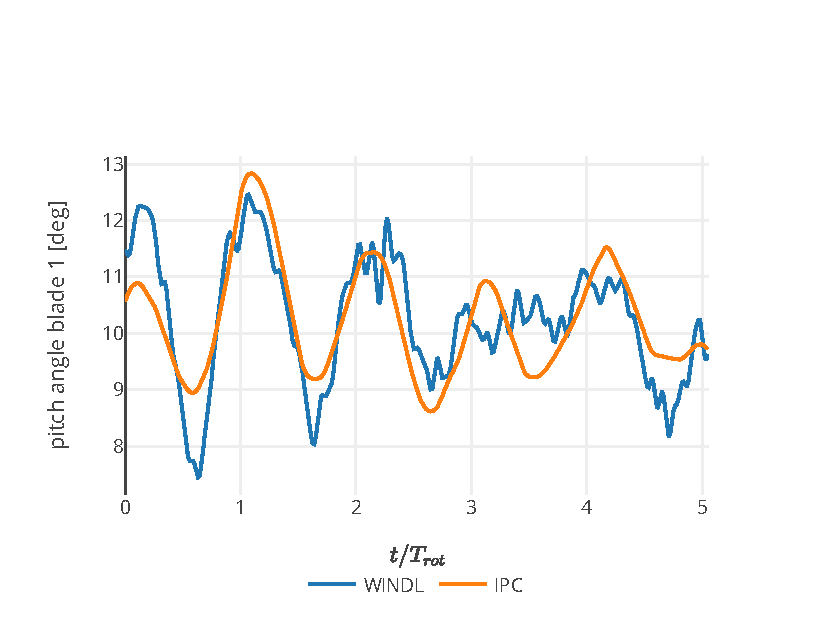
\includegraphics[width=\textwidth]{images/adjusted_pitch_rollout.pdf}
    \caption{Pitch actions over time for mean wind speed 14 m/s}
    \label{fig:adjusted-rollout-pitch}
  \end{subfigure}
  \begin{subfigure}[b]{0.48\textwidth}
      \centering
      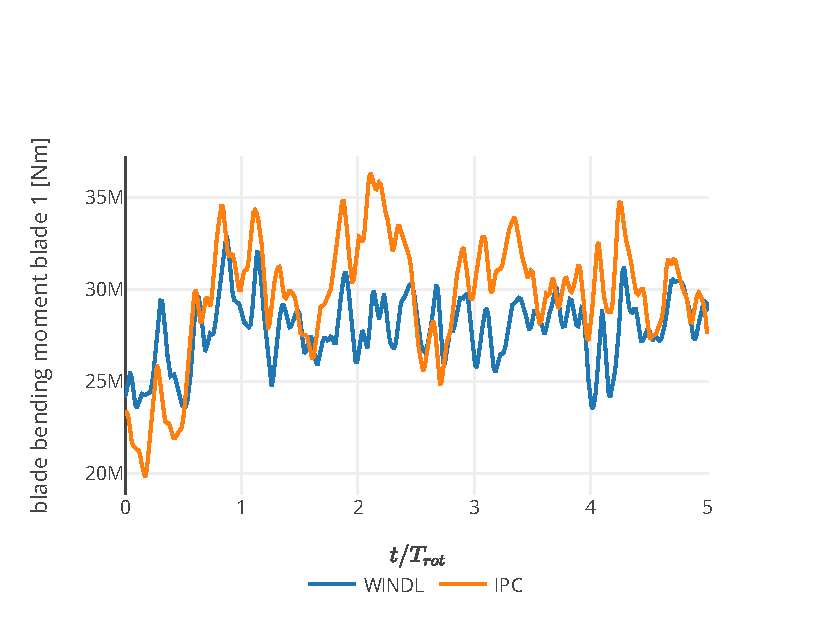
\includegraphics[width=\textwidth]{images/adjusted_lowwind_blade_rollout.pdf}
      \caption{Blade bendings over time for mean wind speed 12 m/s}
      \label{fig:adjusted-rollout-lowwind-blade}
  \end{subfigure}
  \begin{subfigure}[b]{0.48\textwidth}
    \centering
    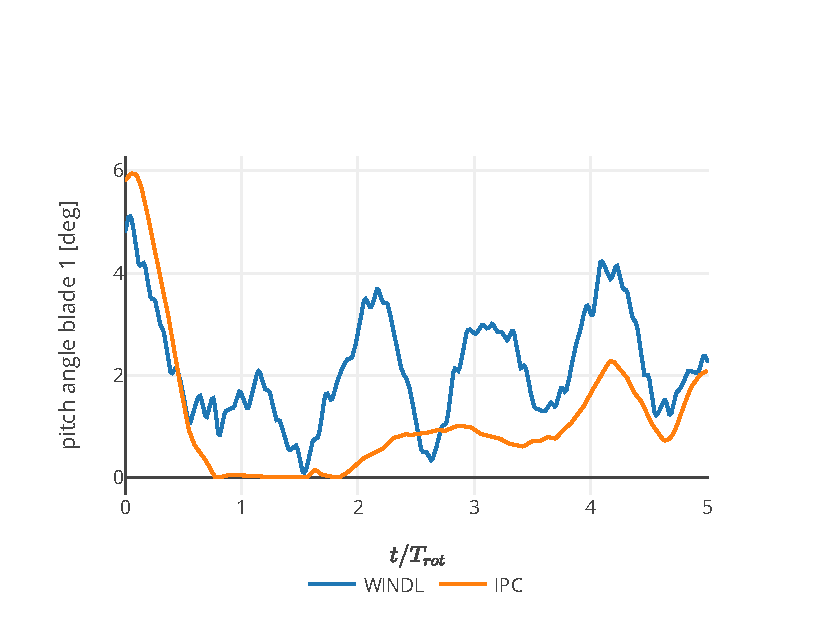
\includegraphics[width=\textwidth]{images/adjusted_lowwind_pitch_rollout.pdf}
    \caption{Pitch actions over time for mean wind speed 12 m/s}
    \label{fig:adjusted-rollout-lowwind-pitch}
  \end{subfigure}
  \caption{Rollouts of the pitch actions and blade bendings for the first blade in two different turbulent wind scenarios, one with mean wind speed 14 m/s and one with 12 m/s. The two other blades are ommitted for clarity.}
  \label{fig:adjusted-rollout}
  % sac-turb-optim-1, data_42, turb_reeval_1430, eval_run 160 (12m/s) and 320 (14m/s)
\end{figure}

Figure \ref{fig:adjusted-rollout} shows two rollouts of pitch actions and the corresponding blade movements of WINDL and the IPC for the same wind scenario. Only the actions of blade one are shown for brevity, as the other two blades behave similarly with a phase offset of 120 degrees. The time axis is plotted in multiples of the rotation time ($t/T_{rot}$). Five rotations are shown, which corresponds to 4.5 seconds of simulation time at rated rotor speed. In the blade bending plots, low amplitudes between high and low bending moments are desired for fatigue load reduction and low maxima are desired for extreme load reduction.

In Subplot \ref{fig:adjusted-rollout-pitch}, the difference of pitch actions between WINDL and the IPC is clearly visible. Similar to the steady wind, WINDL pitches on both low and high frequencies, while the IPC only utilizes a single low frequency. When not necessary, WINDL deactivates the low-frequency pitch activity almost completely as visible between rotation 3 and 4. The corresponding blade bendings in the same time on Subplot \ref{fig:adjusted-rollout-blade} show that this corresponds with a lower bending amplitude, suggesting that some of the IPC loads are induced by the supposedly load minimizing pitching policy. At other times like between rotation 0 and 1, WINDL pitches significantly more aggressively than the IPC, which also results in a bending amplitude reduction. The IPC reactions are strongly lowpass-filtered to improve IPC stability, and consequently it is not able to adjust its actions as dynamically as WINDL does. WINDL shows that is is beneficial to allow nuances in the incoming wind to decide over the amplitude of pitching action.

Subplot \ref{fig:adjusted-rollout-lowwind-pitch} shows a wind scenario where a turbulence dips the mean incoming wind speed below rated speed. The mean wind speed for this scenario is 12 m/s, but through a turbulence, it is reduced past 10.75 m/s for a short period of time. This is the period of time where WINDL has the most significant extreme load reduction. As visible in Subplot \ref{fig:adjusted-rollout-lowwind-blade}, the IPC experiences an extreme load at rotation 2 while WINDL does not. This is due to the different pitching actions as shown in Subplot \ref{fig:adjusted-rollout-lowwind-pitch}. The IPC policy is ramped down to no activity to conserve power, but WINDL pitches quite aggressively, especially around the extreme load at rotation 2. This comes with a loss in power. While in Subplot \ref{fig:adjusted-rollout-pitch}, both policies produce the same amount of power at 10 MW, WINDL has an average power level of 8.96 MW, and the IPC of 9.29 MW across the time shown in Subplot \ref{fig:adjusted-rollout-lowwind-pitch}. 

\begin{figure}
  \centering
  \begin{subfigure}[b]{0.48\textwidth}
      \centering
      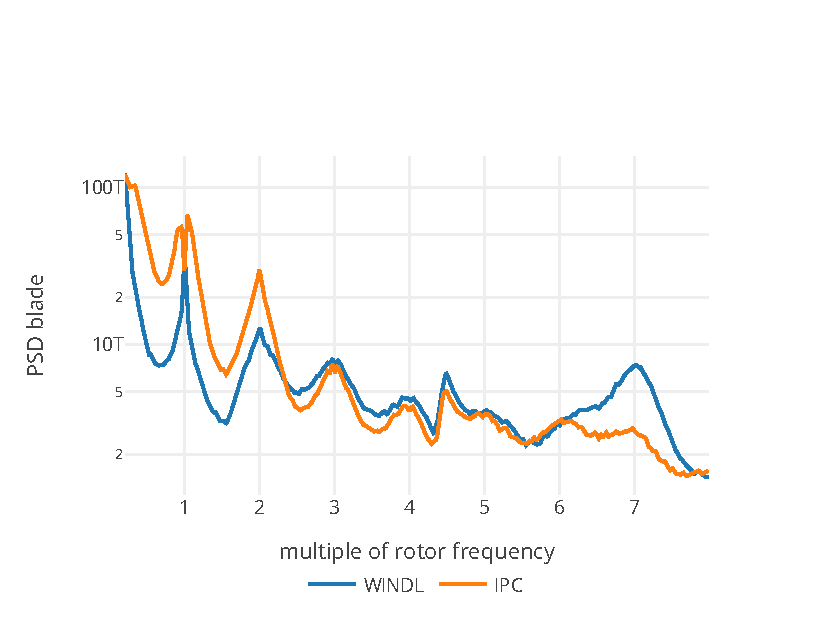
\includegraphics[width=\textwidth]{images/turbulent_psd_blade.pdf}
      \caption{Average blade bending PSD above rated}
      \label{fig:adjusted-psd-blade}
  \end{subfigure}
  \begin{subfigure}[b]{0.48\textwidth}
    \centering
    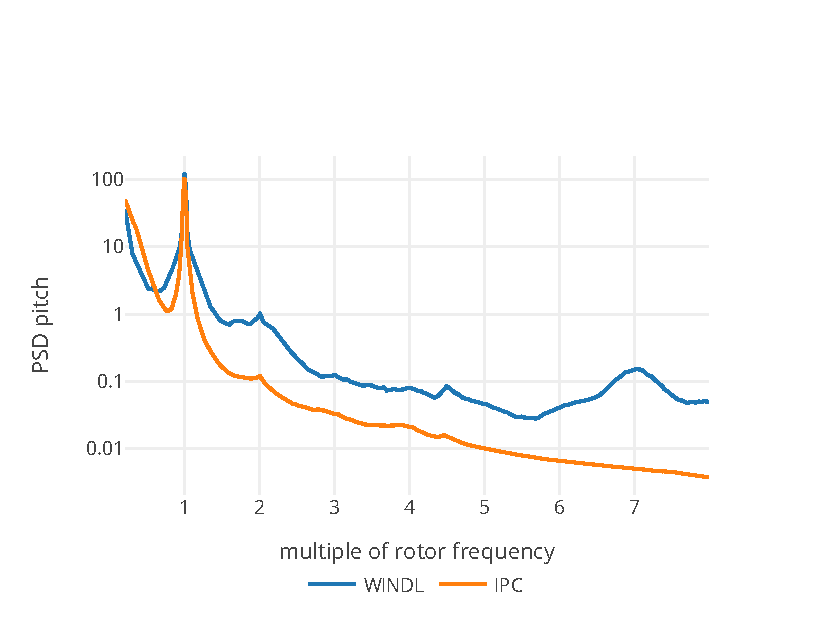
\includegraphics[width=\textwidth]{images/turbulent_psd_pitch.pdf}
    \caption{Average pitch actuation PSD above rated}
    \label{fig:adjusted-psd-pitch}
  \end{subfigure}
  \caption{PSD plots of the pitch actuation and blade bendings, averaged across 648 rollouts above rated and across all three blades. Lower is better.}
  \label{fig:adjusted-psd}
  % sac-turb-optim-1, data_42, turb_reeval_1430, group 2160:
\end{figure}

For further investigation, we plot the \ac{PSD} for both pitch actuation and blade bending averaged across 648 rollouts above rated speed and across all three blades in Figure \ref{fig:adjusted-psd}. This averaging smoothes out turbulence effects and extracts the impact of the policies. Subplot \ref{fig:adjusted-psd-pitch} shows the pitch actuation across the frequency band. The IPC has a sharp spike at the 1p frequency and not much more frequency contents. This is congruent to the behavior below rated speed as shown in Figure \ref{fig:steady-rollout-pitch-psd}. WINDL also exhibits the peak at 1p with a slightly higher maximum value, but with a flatter curvature than the IPC. Actuation around the 1p frequency of the IPC is minimal, while WINDL performs some work between 0.7 and 1.3p. This shows very clearly in the blade PSD in Subplot \ref{fig:adjusted-psd-blade}. Around the 1p frequency, the IPC exhibits two peaks, which are likely the main cause of blade DELs for the IPC. WINDL does not have these peaks around 1p. Also at 2p, WINDL exhibits more pitching action than the IPC and incurs less blade loads. For some reason, WINDL learned to also pitch on the 7p frequency, which seems to be detrimental to blade loads on that side. Such high frequency noise could easily be masked by the noise of the turbulence, and learning the system behavior on that frequency likely poses a challenge, leading WINDL into misbehavior. In contrast to the behavior in the steady wind from Figure \ref{fig:steady-rollout-pitch-psd}, WINDL does not have peaks at 3p, 4p, 5p, and 6p but a continuously lifted pitch band in comparison to the IPC. This is likely the source of the higher pitch loads, together with the slightly higher actuation at 1p. 

\subsection{Discussion}

The IPC idea first presented by \citet{bossanyiIndividualBladePitch2003} introduced a funtamentally different idea than the previous state-of-the-art, the CPC, reducing blade fatigue loads significantly at the cost of some pitch wear. It slowly gains adoption, as the trade-off pays off on some turbines. WINDL shows to be capable of advancing this trade-off even further. With hyperparameters adjusted to the challenges of the turbulent wind, it outperforms the state-of-the-art IPC policy with respect to blade fatigue loads by a similar margin as the IPC outperforms the CPC. Congruent with the switch from CPC to IPC, this does happen at the expense of pitch activity. Furthermore, WINDL shows a reduction of extreme loads, which is partially achieved by trading power production but partially also due to intelligent pitching behavior. 

WINDL outperforms the IPC above rated by 13.5\% lower fatigue loads at the expense of 110\% higher pitch wear. The reduction is comparable to the improvement of switching from a CPC to an IPC, which brings 9.87\% lower blade DELs at the expense of 67.8\% higher pitch wear. Furthermore, WINDL shows a reduction of extreme loads of 5.45\% above rated compared to the IPC, which comes with a loss of power of 0.1\%.

In the turbulent wind setting, WINDL again showed the potential to black-box optimize to a performance level which matches or outperforms model-informed baselines. This requires multiple adjustments of hyperparameters to adjust WINDL to the wind scenario at hand. The need for such hyperparameter adjustments is a set-back to the idea of reinforcement learning to black-box optimize any scenario to perfection and a hindrance to adoptment, as the wind scenarios a turbine will operate in are only partially predictable.

Extreme load reductions are especially relevant around rated speed. WINDL trades some power for lower extreme loads. Whether this is economically feasible is dependent on the turbine model and the possible blade price reduction that goes with it. If this extreme load reduction is not wanted, future work could implement a policy ramp down around rated speed similar to the IPC to prevent power loss. Such a ramp down would increase blade wear and extreme loads but conserve power and pitch wear around rated speed. Future work could also investigate a power penalty in the reward function.

The high performance stems from the ability of WINDL to adapt its behavior to the turbulence at hand based on more information than purely average wind speed or the current blade loads. Through the extraction of knowledge from the entire sensor array and the near past, it decides when to invest pitching actions and when to conserve them. Furthermore, it alleviates extreme loads during temporal wind speed dips below rated by retaining a pitching motion where the IPC ramps down any pitching behavior. Pitch actuation around the 1p frequency and on the 2p frequency lead to a reduction in blade loads on these frequencies, giving WINDL an edge over the IPC in terms of blade wear.


\section{Tuning For The Pitch-blade Trade-off}
\label{section:results-pb-trade-off}

\begin{summary}
In this section, we investigate one of the trade-offs in controller design, the trade between pitch and blade loads. We try different hyperparameter combinations and show that through adjustment of training hyperparameters, the optimization focus can be shifted between the trade-off goals. Counterintuitively, the policy performance is not controlled mainly through the reward function coefficients but through other hyperparameters.
\end{summary}

For this section, we train each hyperparameter combination four times with different seeds up to 500 epochs (approx. 7M environment interactions) in the steady wind scenario or 1500 epochs (approx 40M environment interactions) in the turbulent wind scenario. 

Depending on the wind turbine model, materials, and resource costs, the blades or the pitch system can take a more significant part of the total costs. For smaller turbines, the blades are generally cheaper than the complex pitch system. When scaling turbine size up, the price of the blades rises faster than the price of the pitch system, because the blades have to carry their own weight. Through this trend, larger turbines can benefit strongly from lower blade wear. \cite{stehly2019CostWind2020} Both components are designed such that they last the entire design life-time of the turbine subject to the expected loads, as neither can be replaced easily during operation. Through the choice of a fast-pitching control policy, some blade loads can be mitigated at the cost of higher pitch activity or vice versa. Being able to control this trade-off through controller parametrization allows the control policy to be adapted to the requirements of a large number of wind turbines.

\subsection{Presentation}

\begin{table}
  \centering
  \begin{tabular}{rcc@{\hskip 1.5cm}cc}
    \toprule
    & $\lambdatemp$ & $\lambdaspat$ & $\bdelrel$ & $\pdelrel$ \\
    \midrule
    1 & 0.0 & 0.0 & 0.71 & 1.04 \\
    2 & 0.025 & 0.0 & 0.45 &  1.00 \\
    3 & 0.05 & 0.0 & 0.43 & 1.02 \\
    4 & 0.1 & 0.0 & 0.59 & 0.97 \\
    5 & 0.2 & 0.0 & 0.87 & 0.91 \\
    6 & 0.0 & 0.01 & 0.50 & 1.04 \\
    7 & 0.0 & 0.02 & 0.46 & 1.02 \\
    8 & 0.0 & 0.04 & \textbf{0.42} & 1.02 \\
    9 & 0.0 & 0.08 & 0.46 & 1.00 \\
    
    \midrule
    10 & 0.05 & 0.01 & 0.43 & 1.01 \\
    11 & 0.1 & 0.01 & 0.60 & 0.97 \\
    12 & 0.2 & 0.01 & 0.99 & 0.88 \\
    13 & 0.05 & 0.05 & 0.51 & 0.98 \\
    14 & 0.1 & 0.05 & 0.73 & 0.94 \\
    15 & 0.2 & 0.05 & 1.10 & \textbf{0.87} \\

    
    \bottomrule
  \end{tabular}
  % sac-steady-optim-3 (top half) and sac-steady-optim-2 (bottom half)
  \caption{\acs{IQM}-values for relative performance of WINDL compared to the IPC for different \ac{CAPS} parameter combinations at windspeed 18 m/s and in steady wind. Lower than 1 means WINDL is better than the IPC. Several local optima can be found through adjustment of \ac{CAPS} parameters.}
  \label{table:pb-trade-steady}
\end{table}


Table \ref{table:pb-trade-steady} presents \ac{IQM} values of the relative bDEL and relative pDEL metrics, evaluated at 18 m/s wind speed across four seeds in the steady wind scenario. The best value for each column is shown in bold. Albeit WINDL being trained on the full wind speed range from 10 to 20 m/s, we use a single wind speed in our evaluation to exclude noise across wind speeds for the sensitivity analysis of hyperparameter effects. Another option to find hyperparameter effects would be to perform extensive smoothing across wind speeds and turbulence seeds, which we avoid due to computational costs. We choose this specific wind speed of 18 m/s to be consistent with Figure \ref{fig:steady-rollout}. For a relative DEL value of 1, WINDL matches IPC performance. On lower values, it outperforms it, and on higher values, it performs worse. For each seed, we choose the best model with respect to the arithmetic mean between $\pdelrel$ and $\bdelrel$ among 500 epochs of training.

An intuitive way to approach the pitch blade trade-off is through the $\rcolemanact$ reward penalty, which penalizes pitch travel, and as such, should move the optimum in the reward function towards a more pitch saving policy. In our experiments, we found this to not work well in the steady wind. Using \ac{CAPS} parameters instead is far more stable. In rows 2-5, temporal smoothness regularization not only reduces pitch wear (right column) but also reduces blade wear (left column) up to $\lambdatemp = 0.05$. The same happens for $\lambdaspat$ in rows 6-9, which also reduces both pitch and blade wear up to a certain margin. The optimum at $\lambdaspat=0.04$ produces comparable results as the optimum for $\lambdatemp = 0.05$. The optima from rows 3 and 8 are not easily outperformed by combining the two parameters in rows 10-15. While it is possible to drive pitch wear to lower values than the IPC baseline, this comes at the price of a strong increase in blade wear. The optima from row 3 and 8 are matched with $\lambdatemp=0.05, \lambdaspat=0.01$ in row 10, giving three local optima.

Furthermore, we investigate training stability across random seeds for $\lambdatemp=0.05, \lambdaspat=0.01$, which is the same configuration as used in Section \ref{section:results-steady-fatigue}. The used seeds are different seeds than used for plotting Table \ref{table:pb-trade-steady}, nevertheless values should match row 10. The resulting 95\% confidence interval of bootstrapping \ac{IQM}-values of relative bDEL is $[0.403, 0.444]$ and for relative pDEL it is $[1.000, 1.021]$.


\subsection{Turbulent Wind}

% I want to present:
% Default values like adjusted
% - gamma 0.98, 0.99
% - rcolemanact 0, 0.01, 0.1
% - mask_act [s, no_s]
% And a final run:
% data_1, turb_reeval_1545

\begin{table}
  \centering
  \begin{tabular}{rccc@{\hskip 1.5cm}cc}
    \toprule
    & $\rcolemanact$ & $\gamma$ & Control $c_S$ & $\bdelrel$ & $\pdelrel$ \\
    \midrule
    1 & 0.1 & 0.99 & true & \textbf{0.83} $\pm$ 0.03 & 1.75 $\pm$ 0.09 \\
    2 & 0.1 & 0.99 & false & 0.92 $\pm$ 0.01 & 1.35 $\pm$ 0.09 \\
    3 & 0.1 & 0.98 & true & 0.93 $\pm$ 0.02 & 1.13 $\pm$ 0.06 \\
    4 & 0.1 & 0.98 & false & 0.95 $\pm$ 0.0  & \textbf{1.04} $\pm$ 0.05 \\

    
    % sac-turb-optim-1, filtered to qf_lr 1e-4
    5 & 0.2 & 0.99 & true & \textbf{0.83} $\pm$ 0.03 & 1.88 $\pm$ 0.08 \\
    6 & 0.2 & 0.98 & true & 0.94 $\pm$ 0.02 & 1.07 $\pm$ 0.04 \\

    % sac-turb-optim-2, filtered to caps_lambda_t 0.2

    \bottomrule
  \end{tabular}
  \caption{\acs{IQM}-values for relative performance in the turbulent wind of WINDL compared to the IPC for different hyperparameter combinations. IQMs are calculated across four training seeds and five wind speeds between 12 and 20 m/s. Lower than one means WINDL is better than the IPC. It is possible to trade pitch loads for blade loads, but not by adjusting the reward penalty.}
  \label{table:pb-trade-turbulent}
\end{table}

Table \ref{table:pb-trade-turbulent} presents values of the relative bDEL and relative pDEL metrics for different hyperparameter combinations, evaluated at turbulent wind speeds between 12 and 20 m/s with a resolution of 2 m/s. To account for turbulence noise, values are bootstrapped to a .95-confidence interval and the interval size is denoted after the metric. We train each combination for four random seeds, and for each seed, we choose the best model with respect to $\bdelrel$ among 1500 epochs of training. All unspecified hyperparameters are kept as listed in Table \ref{table:hyperparameters} for the turbulent wind. Note that row 1 exactly matches the hyperparameter set from Table \ref{table:hyperparameters} and is evaluated thoroughly in Section \ref{section:results-adjusted}. Slight differences in results between row 1 of Table \ref{table:pb-trade-turbulent} and Table \ref{table:improvements-bdelopt} are due to the lower evaluation resolution used to produce the table in this section.

In rows 3, 4, and 6, a lower discounting factor is used compared to the adjusted WINDL from row 1. This consistently results in higher blade DELs but lower pitch DELs. In row 4, pitch DELs are just 4\% above IPC level with 5\% lower blade DELs. In rows 2 and 4, the controller can not change $c_S$; it is kept constantly at zero. Hence, it can not apply a collective offset angle. Prohibiting this brings lower pitch loads as expected, but at the cost of higher blade loads. The difference in $\bdelrel$ between row 1 and 2 is especially pronounced, reducing the improvement from 17\% to 8\%. In row 5 and 6, a higher penalty for pitch travel is used. Despite the higher pitch penalty, row 5 exhibits the same blade DELs as row 1 with worse pitch DELs. Row 6 yields results closer to expectations, with slightly higher blade DELs and slightly lower pitch DELs than row 3.


\subsection{Discussion}

We show the pitch-blade trade-off to be controllable through the choice of hyperparameters. In the steady wind, these are most notably the \ac{CAPS} parameters $\lambdatemp$ and $\lambdaspat$, while in the turbulent wind it is the discounting factor $\gamma$ and the ability to control $c_S$.

While in the steady wind, trading pitch and blade wear is possible roughly one-on-one, we found the pitch blade trade-off to work differently in the turbulent wind. Here, small relative reductions in blade wear required high trades on the pitch side. We attribute this to the fact that in the turbulent wind, blade wear is mostly dominated by the turbulences themselves, and a load minimizing policy only has a slim margin to counteract that.

The intuitive solution of changing the pitch travel penalty in the reward function does not yield satisfactory results. This is congruent to the findings of \citet{mysoreRegularizingActionPolicies2021}, which claim smoothness penalties in the reward function to not work well in practice. However, not including the reward function in the turbulent wind did not play out well either. Section \ref{section:results-reward} goes into detail on the interplay of the reward function components.

Finding a globally optimal hyperparameter combination is a non-trivial task, as multiple local optima are to be expected. Hence, adjusting the pitch-blade trade-off is compute-intensive, but possible. Performing at least some hyperparameter optimization is highly beneficial, as for good choices, hyperparameters can benefit both blade and pitch wear. With sensible hyperparameters, it is possible to find a policy that performs within 10\% of the upper bound in a single training. 

Investing more compute through different random seeds can yield a bonus and is highly recommendable to smooth sampling noise during hyperparameter effect estimation. A difference in performance of up to 10\% can be observed by utilizing a different random seed, and especially when fine-tuning hyperparameters, the possibility of a lucky seed should be factored out. 

We require ca. 1500 CPU-hours for a steady training run to 750 epochs and ca 5000 CPU-hours for a turbulent training run to 1500 epochs, which is well within the scope of capabilities of modern HPC clusters. Because the training is only necessary once per turbine model, we estimate that the investments into compute budget are economically feasible for wind turbine development and will not hinder \ac{WINDL} adoption.

Through the possibility of adjusting the pitch-blade trade-off, WINDL is suitable to optimize a wider array of turbines. Turbine installations that do not need such a high blade load relief as brought by the policy from Section \ref{section:results-adjusted} can still benefit from a WINDL variant with tweaked hyperparameters. In contrast to interpretable and relatively deterministic parameter changes on IPC methods that can adjust these approaches to trade differently, the trade-off on WINDL is controlled through hyperparameter changes. The final policy performance of a new hyperparameter set can not be perfectly predicted, hence a grid search is necessary if a specific point in the trade-off spectrum is targeted.

\section{Generalization Between Wind Scenarios}
\label{section:results-transfer}

\begin{summary}
In this section, we measure generalization performance of the policies from previous sections by evaluating them in a wind scenario unseen during training. We show that neither the checkpoint from the steady wind generalizes well to the turbulent wind scenario nor vice versa. We conclude that this limitation brings the need for meticulous policy evaluation.
\end{summary}

Optimally, a policy trained in one wind scenario generalizes to unseen wind scenarios and still performs reasonably. If a real-life wind scenario is missing during training and evaluation, bad generalization performance can result in poor performance and damage to the turbine. While current turbulence models are well researched and standartized \cite{internationalelectrotechnicalcommissionIEC61400120192019}, missing out on a single edge case can potentially trigger unwanted behavior on a strongly overfitting policy. Reinforcement learning is known to struggle with generalization \cite{cobbeQuantifyingGeneralizationReinforcement2019}. In contrast to supervised learning, generalization performance of reinforcement learning algorithms is typically not measured in publications \cite{mnihPlayingAtariDeep2013,haarnojaSoftActorCriticOffPolicy2018,fujimotoAddressingFunctionApproximation2018}. While the supervised field of machine learning is strongly concerned with overfit, reinforcement learning mainly measures bare fit.

\subsection{Steady To Turbulent}

\begin{figure}
  \centering
  \begin{subfigure}[b]{0.48\textwidth}
      \centering
      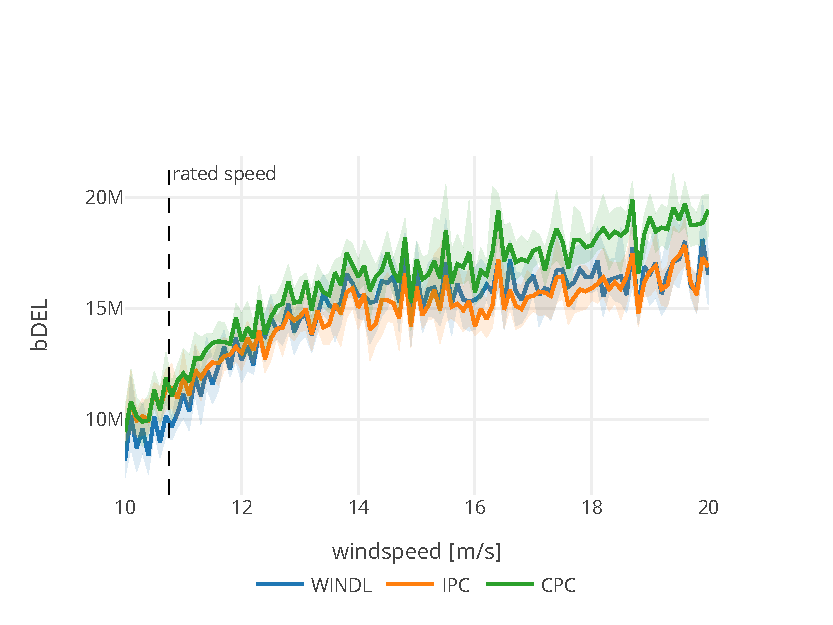
\includegraphics[width=\textwidth]{images/transfer_turbulent_bdel.pdf}
      \caption{blade-DELs against windspeed}
      \label{fig:transfer-turbulent-bdel}
  \end{subfigure}
  \begin{subfigure}[b]{0.48\textwidth}
      \centering
      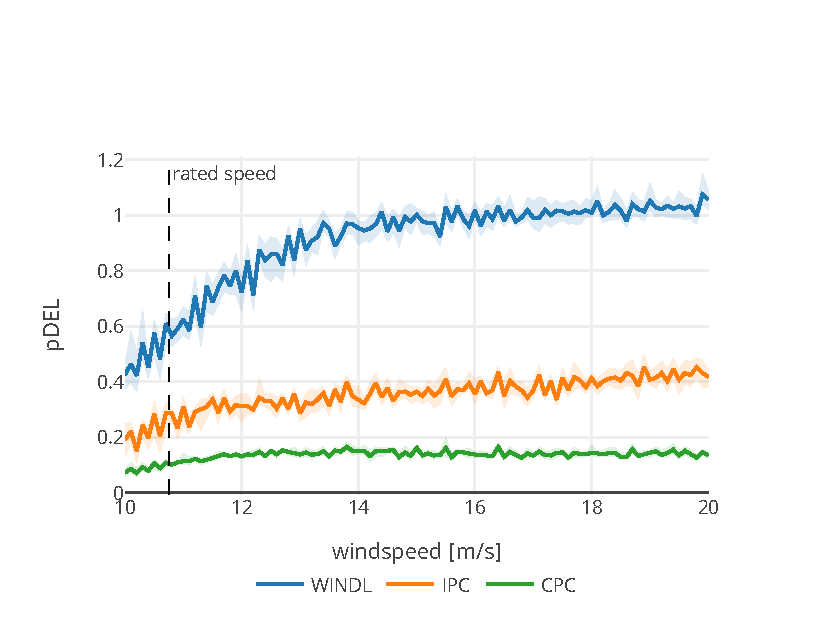
\includegraphics[width=\textwidth]{images/transfer_turbulent_pdel.pdf}
      \caption{pitch-DELs against windspeed}
      \label{fig:transfer-turbulent-pdel}
  \end{subfigure}
  \caption{The transfer performance of a model trained in the steady wind on a turbulent wind scenario, compared to IPC and CPC performance. Lower is better.}
  \label{fig:transfer-turbulent}
  % sac-steady-final, data_0, turb_reeval_468
\end{figure}

We measure the generalization performance of the best performing model from the steady wind (see Section \ref{section:results-steady-fatigue}) by evaluating it in the turbulent wind scenario. Note that the model has never seen a turbulent wind scenario during training. In Figure \ref{fig:transfer-turbulent}, we run WINDL on eight different turbulent seeds per wind speed for wind speeds between 10 and 20 m/s with a resolution of 0.1 m/s. For each metric, we plot a solid line for the mean value of performance across the turbulent seeds and a thin area around it for the bootstrapped 90\% confidence interval of these mean values. For both plots, lower values are better.
% Subfigure \ref{fig:transfer-turbulent-extreme} presents extreme values, which are calculated as the 99\% quantile value for blade bending moments. Subfigure \ref{fig:transfer-turbulent-rollout} presents an example rollout from the evaluation. 

While blade DELs in Subfigure \ref{fig:transfer-turbulent-bdel} largely match IPC performance, pitch wear values in Subfigure \ref{fig:transfer-turbulent-pdel} are on average 2.61 times as high as the IPC performance and 6.69 times as high as the CPC. In Figure \ref{fig:steady-sweep}, the same policy was able to outperform in terms of blade DELs while exhibiting the same pitch DELs. We also calculate extreme load values as the $.99$-quantile value for blade bending moments across the rollout. We find that WINDL exhibits 2.7\% higher extreme loads than the IPC but 7.55\% lower extreme loads than the CPC. 

\subsection{Turbulent To Steady}

\begin{figure}
  \centering
  \begin{subfigure}[b]{0.48\textwidth}
      \centering
      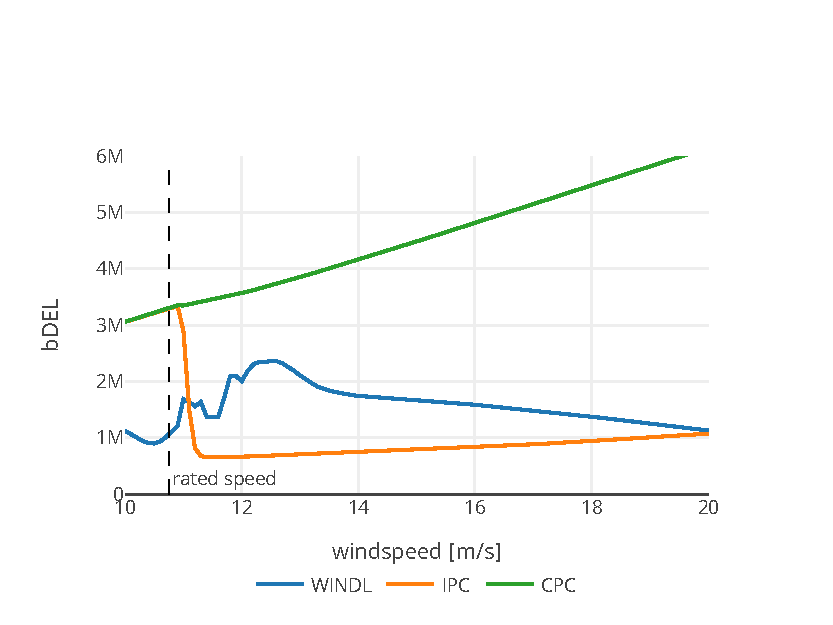
\includegraphics[width=\textwidth]{images/transfer_steady_bdel.pdf}
      \caption{blade-DELs against windspeed}
      \label{fig:transfer-steady-bdel}
  \end{subfigure}
  \begin{subfigure}[b]{0.48\textwidth}
      \centering
      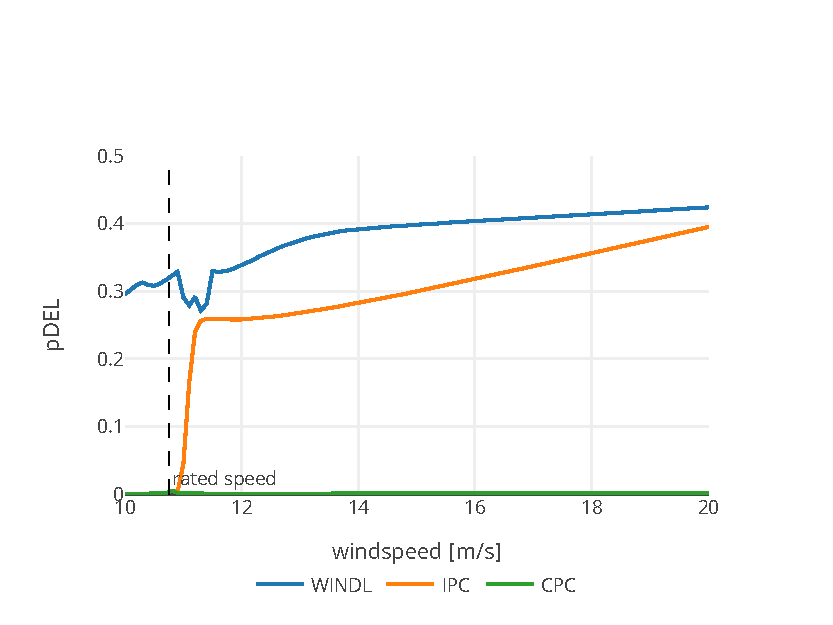
\includegraphics[width=\textwidth]{images/transfer_steady_pdel.pdf}
      \caption{pitch-DELs against windspeed}
      \label{fig:transfer-steady-pdel}
  \end{subfigure}
  \caption{The transfer performance of a model trained in the turbulent wind on a steady wind scenario, compared to IPC and CPC performance. Lower is better.}
  \label{fig:transfer-steady}
  % sac-turb-optim-1, data_42, steady_reeval_1430
\end{figure}

We measure the generalization performance of the adjusted model from the turbulent wind (see Section \ref{section:results-adjusted}) by evaluating it in the steady wind scenario. Note that the model has never seen steady wind during training. In Figure \ref{fig:transfer-steady}, we run WINDL on all wind speeds between 10 and 20 m/s with a resolution of 0.1 m/s. For both plots, lower values are better.

As visible in Subplot \ref{fig:transfer-steady-bdel}, the transfer-evaluated model performs worse than the IPC in terms of blade fatigue loads but better than the CPC. Above rated from 12-20 m/s, it produces 101\% more blade fatigue loads than the IPC but 65\% less than the CPC. At the same time, it exhibits higher pitch wear as visible in Subplot \ref{fig:transfer-steady-pdel}. Above rated, pitch wear is 25\% worse than the IPC. A phenomenon occurs at 11m/s, the onset speed of the torque controller, where both metrics show a dent. In the turbulent wind, transitioning this operating area happened only for small time periods during a gust, while resting at this operating area likely presents unseen challenges to the controller.

Around rated speed between 10 and 12 m/s, WINDL produces lower blade fatigue loads than both the IPC and the CPC, as visible in Subplot \ref{fig:transfer-steady-bdel} on the left side. Notably, it also produces lower fatigue loads than the WINDL policy that was trained in the steady wind in this area when compared to Figure \ref{fig:transition-bdel}. This comes at the price of a significant power loss. While the WINDL policy trained in the steady wind only loses 0.6\% power in the 10 - 12 m/s range, the policy trained in the turbulent wind loses 2.8\% compared to IPC and CPC. The policy trained in the steady wind did not have the capability of trading as much power for blade loads as the policy from the turbulent wind, as the hyperparameter set forbids the steady wind policy to set $c_S$ - the constant offset action. The turbulent policy can freely trade power for blade loads by setting $c_S$ to its maximum value.

\subsection{Discussion}
\label{section:results-transfer-discussion}


WINDL does not transfer well between wind scenarios. In the steady-to-turbulent direction, blade wear remains sensible, but pitch wear is far above the values of the IPC. In the other direction from turbulent to steady, WINDL produces worse pitch and blade wear than the IPC baseline above rated and loses significant amounts of power around rated. While both behaviors would likely not lead to immediate destruction of the turbine, operating a WINDL policy in a wind scenario for which it was not trained is not advisable.

The difference between the steady and turbulent wind scenarios is immense. We do not expect a controller to learn the extreme dynamics of turbulences only from the steady wind. Neither was our expectation for the controller to learn the gentle adjustments necessary to outperform in the steady wind while being subjected to heavy turbulences. However, the underlying dynamics of the turbine are the same, so generalization is not impossible. The shown case could be the most difficult generalization task for wind turbine environments. We do not evaluate generalization tasks that could be easier to solve, such as generalizing from lightly turbulent to strongly turbulent wind where stochastic elements are present in both scenarios.

We expect slightly better results upon utilization of generalization techniques such as dropout or deep neural nets, but we do not expect a drastic improvement. \citet{cobbeQuantifyingGeneralizationReinforcement2019} have shown common ML generalization tweaks to work, but did not record massive improvements. For their causal ladder model, \citet{pearlCausalInferenceStatistics2009} even prove that correct interventions generally require knowledge of the underlying causal model of the environment, as purely associational knowledge can be confounded. The knowledge encoded in the Q-function is purely associational. In a wind turbine, all parts are connected together, and as such, every part is a potential confounder for every other. For example, it is possible to excite a harmonic frequency of a part in a very specific scenario, which did not occur in all previously seen scenarios. Without the knowledge of the underlying model, this is impossible to predict. Additionally, relationships are often non-linear or stochasic, forming a generally difficult environment. The combination of the difficult wind turbine environment and the absence of modeling in our framework make good generalization performance unrealistic to achieve.

Modern wind turbine simulations are accurate models of the dynamics of a wind turbine \cite{martenQBladeModernTool2020}. Furthermore, there is at least some knowledge on the stochastic nature of turbulences \cite[Chapter 2.6.1]{burtonWindEnergyHandbook2011}. These models could be used for a model-based reinforcement learning approach in future work.

For a real-world application of the model-free WINDL, this means that an exhaustive evaluation set is crucial. All types of wind scenarios must be present in evaluation to build enough confidence in the performance of the algorithm, as relying on generalization performance is not advisable. An example of this benchmark could be the IEC 61400-1 standard \cite{internationalelectrotechnicalcommissionIEC61400120192019}, which defines a set of design load cases for a turbine. Furthermore, stability guarantees are a crucial argument for real-world application in addition to empirical performance. Proving stability guarantees is impossible without a model of the environment, and hence a switch to model-based RL methods such as the approach by \cite{berkenkampSafeModelbasedReinforcement2017} could be an option.

\section{Reward Function}
\label{section:results-reward}

\begin{summary}
This section investigates the suitability of the reward function to represent the quantities of interest. We investigate the components of the reward functions and find that they relate to their respective quantities of interest. Furthermore, we show that the magnitude of these components is not congruent with the effect they have on final policy performance. 
\end{summary}

We evaluate the training from Section \ref{section:results-adjusted}, which trains an adjusted policy in the turbulent wind to 1500 epochs (36M environment interactions). We only show the first part of the training to 10M environment interactions to improve the readability of the plots.

We introduce the optimization aims in Section \ref{section:background-optimization-aims} and describe how the reward function is a heuristic for these optimization aims in Section \ref{section:approach-reward-shaping}. While it would be mathematically possible to optimize DEL metrics directly, we use a reward function based on heuristics that can be computed for every timestep to give instantaneous feedback. It is desirable for these heuristics to exhibit optima in the same place of the parameter space as the underlying physical wear process. Hence, we expect the components of the reward function to reflect DEL metrics. Where the DEL metric is high, a high penalty should be applied to incentivize different behavior.

\subsection{Presentation}

\begin{figure}
  \centering
  \begin{subfigure}[b]{0.48\textwidth}
      \centering
      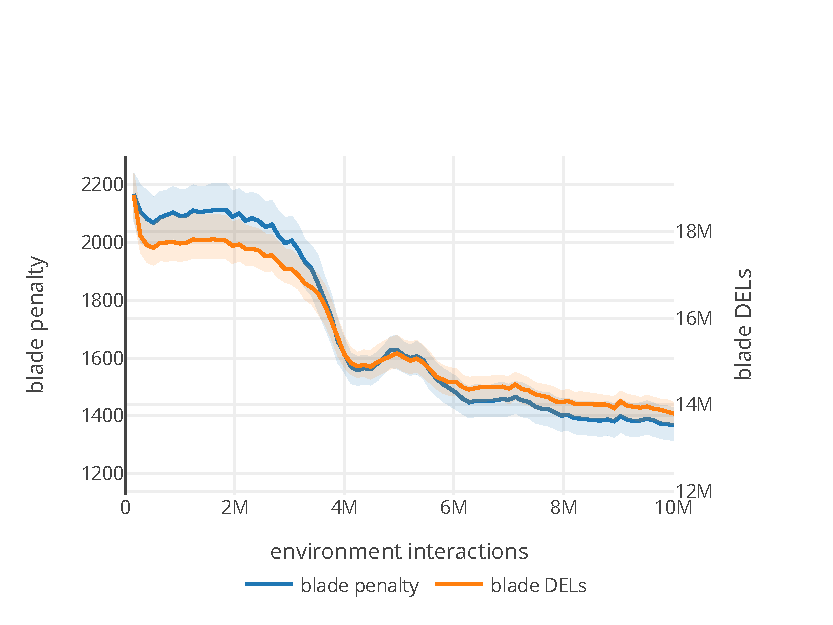
\includegraphics[width=\textwidth]{images/reward_analysis_blade.pdf}
      \caption{Blade penalty and DELs over training time}
      \label{fig:rc-blade}
  \end{subfigure}
  \begin{subfigure}[b]{0.48\textwidth}
      \centering
      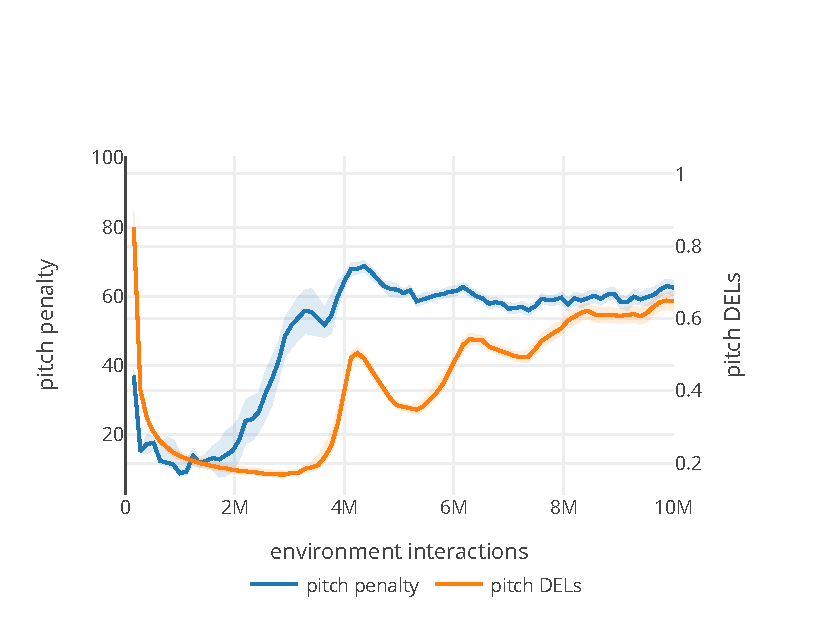
\includegraphics[width=\textwidth]{images/reward_analysis_pitch.pdf}
      \caption{Pitch penalty and DELs over training time}
      \label{fig:rc-pitch}
  \end{subfigure}
  \caption{Reward composition compared to DEL development over training time. The reward penalties for blades and pitch loosely match the DEL metrics of their component}
  \label{fig:rc}
  % sac-turb-optim-1, [], {'deterministic': True, 'mask_act': 'coleman-no-torque-s', 'discount': 0.99, 'qf_lr': 1e-4}, windspeed >= 12
\end{figure}

Figure \ref{fig:rc} shows the reward components over the course of a training plotted together with the relative DEL metrics of the same training run. The value plotted as blade penalty is the norm of the Coleman transformed blade bendings: $\rcoleman \sqrt{\tilde{c_s}^2 + {c_d}^2 + {c_q}^2}$. The value plotted as pitch penalty is calculated as $\rcolemanact \sqrt{{c_S}^2 + {c_D}^2 + {c_Q}^2}$. Note that both penalties are \textit{subtracted} from the reward function, so the agent optimizes towards lower values. Because of the different scales of reward components and DELs, two y-axes are used with the leftmost one corresponding to the reward component and the rightmost one to the DEL value of that turbine component. The constant offset $\rconst=1$ is omitted for brevity. Both plots show \ac{IQM} performance across eight wind speeds between 10 and 20 m/s and four training runs with different random seeds for each point on the x-axis. 

The pitch and blade penalty have different orders of magnitude. Blade penalties are around 20 times higher than pitch penalties. Despite the difference of one magnitude between the pitch reward and the blade reward, the pitch reward has an impact on final policy behavior. We observed that especially with lower discounting factors, increasing $\rcolemanact$ further lead to policies not doing anything in our hyperparameter search because the pitch penalty had a too great influence. The value shown here incentivizes pitch saving behavior in comparison to the naive training as shown in Section \ref{section:results-naive-turbulent}.

The curvature in the pitch penalty plot in Subfigure \ref{fig:rc-pitch} loosely matches the mirror of the curvature of pitch DELs. At 4M environment interactions, a peak in pitch DELs is accompanied by a small peak in pitch penalty, suggesting that this peak was captured by the reward function. An upwards trend with a small downwards peak in pitch penalty from 2M to 3.5M environment interactions is not visible in the DEL plot, suggesting that a phenomenon penalized by the reward function is not relevant for pitch DELs. Even though the pitch penalties stay relatively level above 4M environment interactions, pitch DELs increase in waves, suggesting another mismatch between pitch DELs and the pitch reward component.

The blade penalty as shown in Subfigure \ref{fig:rc-blade} very closely matches blade DELs. Peaks in both direction show both in the reward component and the DEL metric, suggesting that the reward component is a good heuristic for blade DELs. The general trend of blade DELs is downwards, meaning towards a better-performing policy with respect to the primary optimization aim.

\subsection{Discussion}

Counter to expectations, the algorithm does not weigh the pitch and blade component of the reward function equally. A pitch penalty one order of magnitude below the blade penalty is enough to incentivize pitch saving behavior, while increasing the pitch penalty further does not reduce pitch wear as shown in Section \ref{section:results-pb-trade-off}. We attribute this to the learnability of the two components. While pitch wear is directly caused by policy actions, blade wear is mostly caused by turbulence. Hence, learning the pitch penalty is easier, and a pitch penalty one order of magnitude smaller is sufficient to incentivize a behavioral change.

While the pitch penalty seems to only loosely match pitch DELs, the blade penalty reflects blade DELs well. This might partially explain the different success levels on minimizing blade DELs and pitch DELs. Each of the two penalties is constituted of the norm of a three-element vector, and the influence of the individual vector elements on these plots is not shown. While mainly penalizing pitch and blade wear, the reward function also serves to inhibit local maxima as described in Section \ref{section:approach-reward-shaping} through the inclusion of the $\tilde c_s$ and $c_S$ components. Inhibiting local maxima can cause movement in the penalty components that is not reflected in DELs. 

In total, our chosen reward function is a suitable metric for optimization through reinforcement learning. The instantaneous feedback enables easier learning across long trajectories, it does not exhibit local maxima that can be exploited, and it matches the optimization quantities at hand. Accumulating six signals into one does not throw off the Q estimation process, and enough signal-to-noise ratio is retained to train a Q function approximator.

In this chapter, we omit results from experimenting with other reward functions. We tried combinations of penalties for raw pitch travel, raw blade bendings, power loss, rotational speed fluctuation, exceeding maximum rotational speed, tower vibrations, and raw tower bendings. After lengthy searches for suitable coefficients, we settle for the Coleman-based reward function due to its simplicity.

\section{RL Algorithm Components}
\label{section:results-rl-components}

\begin{summary}
This section goes into detail on the different components of the reinforcement learning algorithm. We show the interaction of the Q-function and policy in general and investigate raw neural network outputs in detail. We find that the Q-function is flatter than expected within the action space bounds, which could be caused by the complex state domain of the wind turbine environment. Furthermore, we are unable to extract insights into the knowledge of the network from Q outputs. 
\end{summary}

We evaluate the training from Section \ref{section:results-adjusted}, which trains an adjusted policy in the turbulent wind to 1500 epochs (36M environment interactions).

As described in Section \ref{section:background-sac}, different components of the actor-critic algorithm interact to optimize the quantity of interest: expected discounted return. The critic, which is called Q-function throughout this work, aims to fit expected return for arbitrary states and actions. The actor, which is called policy throughout this work, aims to find the action that maximizes the Q-value for a given state. The Q-function is trained by using the Bellman backup from Equation \ref{eq:bellman-backup} in a recursive manner with separate target networks. To counteract overestimation bias, two Q-functions are used. The policy is trained by deriving a gradient through the more conservative of the two Q-functions, leading the policy towards a maximum in the Q-function curvature.

\subsection{Training Process}

\begin{figure}
  \centering
  \begin{subfigure}[b]{0.48\textwidth}
      \centering
      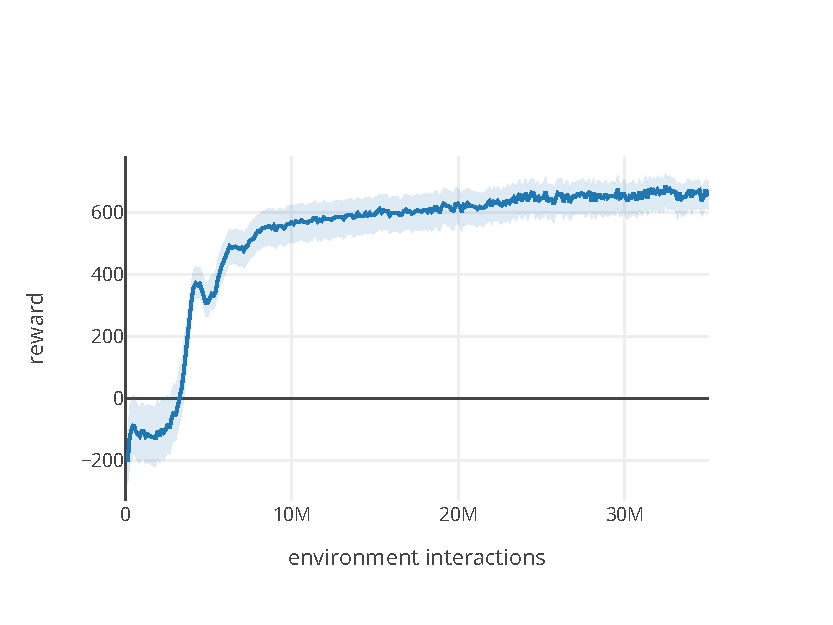
\includegraphics[width=\textwidth]{images/algocomps_reward.pdf}
      \caption{Reward over training time}
      \label{fig:training-reward}
  \end{subfigure}
  \begin{subfigure}[b]{0.48\textwidth}
      \centering
      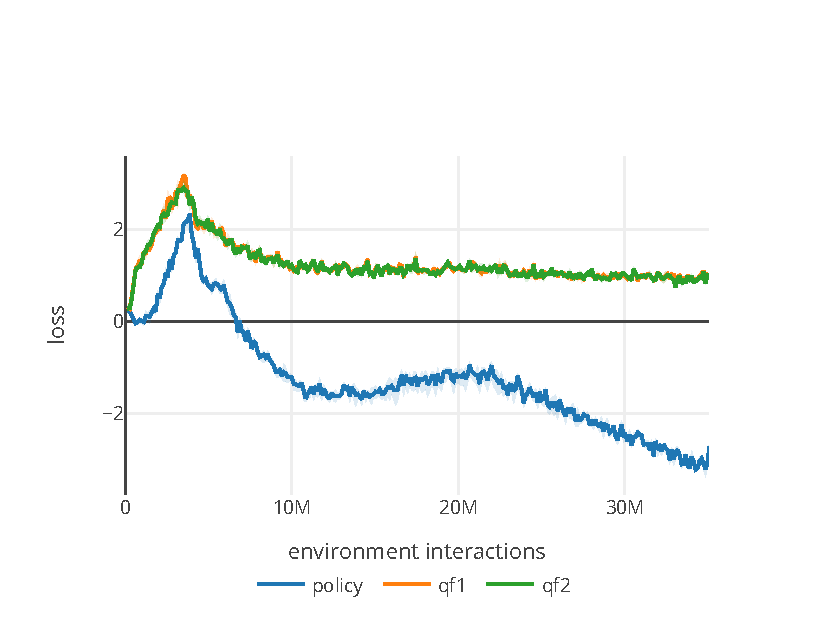
\includegraphics[width=\textwidth]{images/algocomps_losses.pdf}
      \caption{Losses over training time, policy loss scaled by a factor of 0.2 to fit the plot axis}
      \label{fig:training-loss}
  \end{subfigure}
  \caption{Reward and loss development over training time}
  \label{fig:training}
  % sac-turb-optim-1, [], {'deterministic': True, 'mask_act': 'coleman-no-torque-s', 'discount': 0.99, 'qf_lr': 1e-4}, windspeed >= 12, policy loss magnified * 0.2
\end{figure}

Figure \ref{fig:training} shows the losses of the Q-functions and policy over the training time, together with the average reward of the policy. The reward function is discussed in Section \ref{section:results-reward}, where the reward composition for the first 8M environment interactions is shown. Note that the policy loss is not a loss in the traditional sense of a difference between predictions and target values. It is the output of the Q-function for the action generated by the policy, meaning it is an estimate of the return that the policy would achieve with the current action, as shown in Equation \ref{eq:soft-policy-update}. Because the deep learning library in use (pytorch), only supports gradient \textit{descend} while the optimization aim in Equation \ref{eq:soft-policy-update} is a \textit{maximization} objective, the output is multiplied by -1. Hence, negative policy loss stems from a positive Q estimate.

In the first part of the training to 8M environment interactions, the reward function changes most, whereas after 8M environment interactions, it slowly rises to its plateau value of around 650. Around 4M environment steps, a bump in the reward function is visible. Also, around 4M environment steps, both the policy and Q-function losses peak. The policy loss decreases with a stagnation between 13M and 21M environment interactions, while the Q-function losses stagnate.

We observe a peak similar to the one at 4M environment steps throughout all of our training process. Different hyperparameter choices move, but do not remove the period of rising losses at the beginning. This peak coincides with a bump in the reward function, where performance degrades for a short period of time. We investigate this bump and find a strong correlation with policy entropy - the higher the starting entropy target $\alpha$, the more pronounced this bump is.

We believe the exploration strategy to be the cause for this bump. To enable exploration, the policy has a gaussian noise component that is maximized through the maximum-entropy framework. This gaussian noise component is detrimental to the wind turbine, as the turbine reacts to the noise applied to it. The effect of this noise is not captured by the Q-function until around 4M interactions, when the negative effect of entropy is starting to be modeled. Earlier modeling of the negative effect is inhibited by the maximum-entropy framework, which incentivizes \textit{maximal} entropy that counters the \textit{minimal} entropy, which is optimal for the wind turbine. Only when policy performance can not be optimized through other means, the algorithm starts to shift attention to the entropy part. From then on, policy performance becomes slightly better with the decreasing $\alpha$ component. The exploration-exploitation trade-off is especially tricky in wind turbine reinforcement learning, as entropy is required for exploration to find better policies, but having entropy causes worse policies. Learning to distinguish between these two counteracting causes is sample-intensive and requires 4M environment interactions. For comparison, \citet{haarnojaSoftActorCriticOffPolicy2018} only train to 3M interactions to solve most gym environments.

\subsection{Q-Function Curvature}

We observe a phenomenon where most of the Q-Function curvature lies outside of the action space.

\begin{figure}[hbt]
  \centering
  \begin{subfigure}[b]{0.48\textwidth}
      \centering
      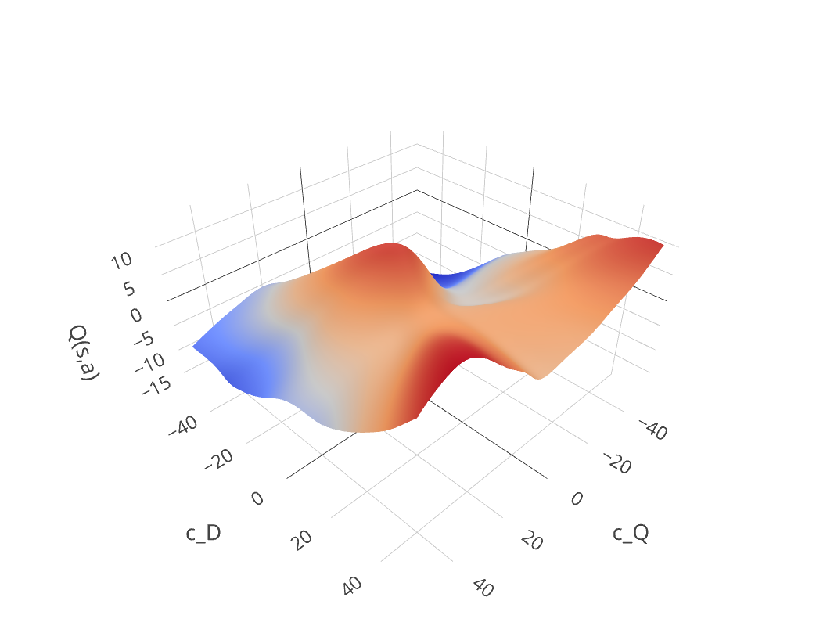
\includegraphics[width=\textwidth]{images/frame_zoomout.pdf}
      \caption{Q-function zoomed out for t=0}
      \label{fig:qf-zoom}
  \end{subfigure}
  \begin{subfigure}[b]{0.48\textwidth}
    \centering
    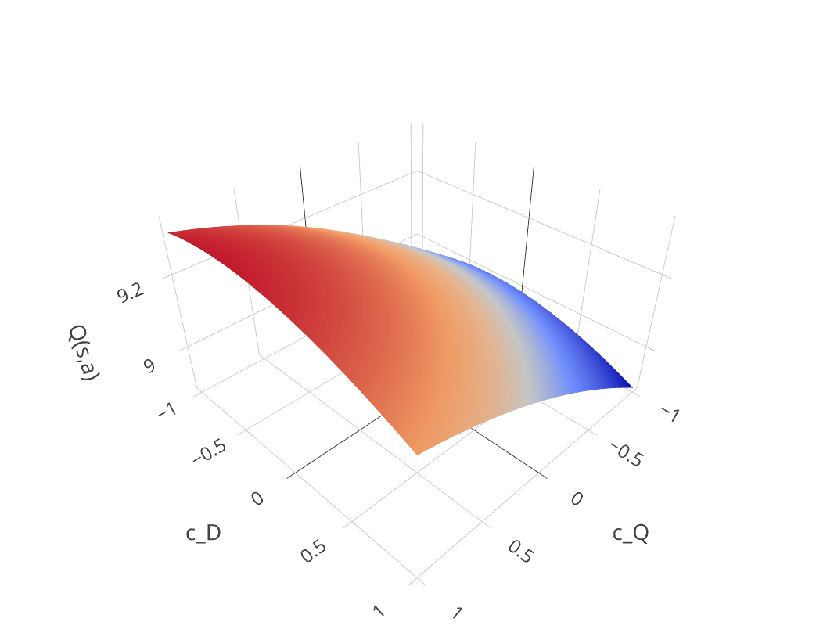
\includegraphics[width=\textwidth]{images/frame_0.pdf}
    \caption{Q-function at t=0}
    \label{fig:qf-t0}
    % traj_idx 879
  \end{subfigure}
  \begin{subfigure}[b]{0.48\textwidth}
    \centering
    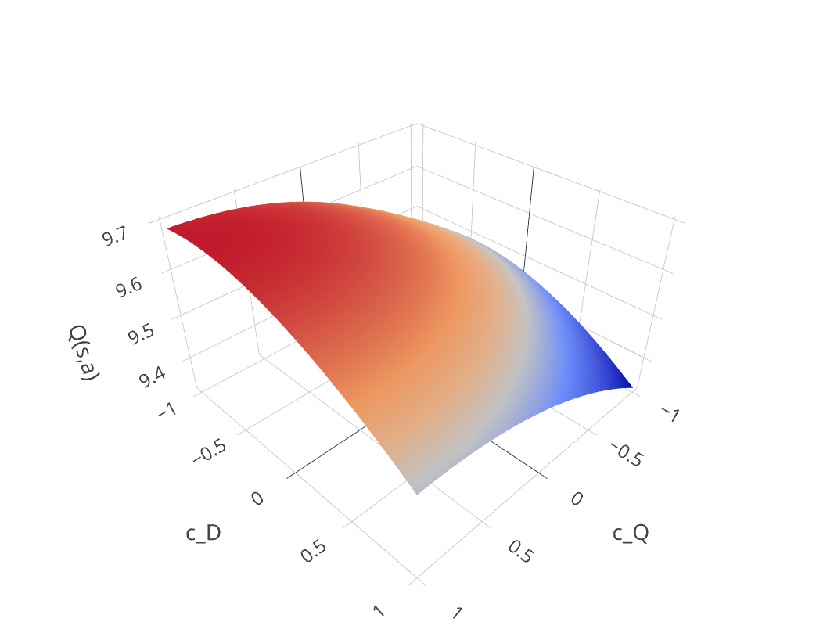
\includegraphics[width=\textwidth]{images/frame_1.pdf}
    \caption{Q-function at t=1}
    \label{fig:qf-t1}
    % traj_idx 880
  \end{subfigure}
  \begin{subfigure}[b]{0.48\textwidth}
    \centering
    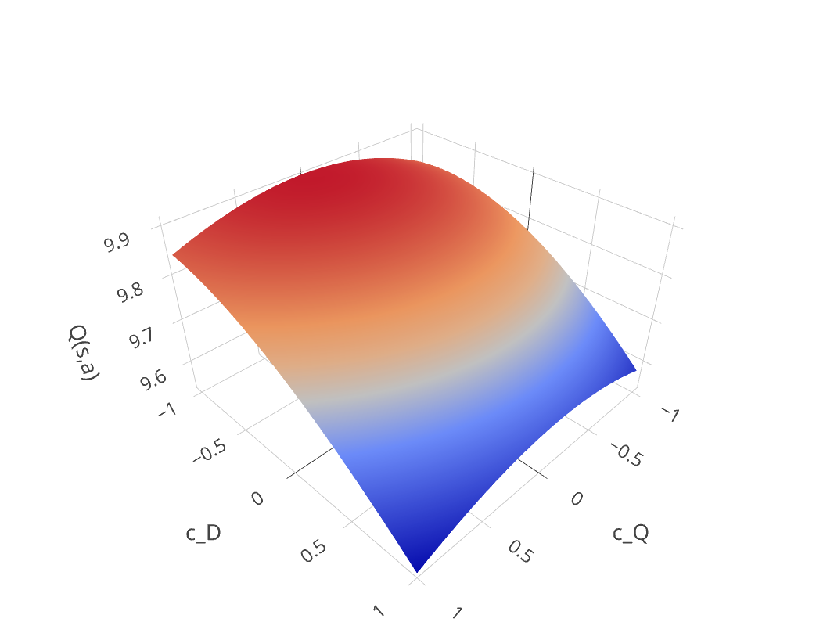
\includegraphics[width=\textwidth]{images/frame_2.pdf}
    \caption{Q-function at t=2}
    \label{fig:qf-t2}
    % traj_idx 881
  \end{subfigure}
  \caption{Q-function curvature across two action space dimensions $c_Q, c_D$}
  \label{fig:qf}
  % sac-turb-optim-1, data_1, eval-1545, eval run 2
\end{figure}

Figure \ref{fig:qf} shows the Q-function values across two dimensions of the action space, $c_Q, c_D$. Section \ref{section:approach-postprocessing} describes these two to be the pitch action difference across the tilting and yawing axes of the rotor plane. In Subplots \ref{fig:qf-t0} \ref{fig:qf-t1} \ref{fig:qf-t2} they are constrained to their allowed range before postprocessing of [-1, 1], while in Subplot \ref{fig:qf-zoom} the Q-function is evaluated for hypothetical actions in the range [-50, 50]. Note that during training, the Q-function has only seen the range [-1, 1]. Subplots \ref{fig:qf-t0} \ref{fig:qf-t1} \ref{fig:qf-t2} show the original Q-function as used during policy optimization for three consecutive time steps.

In the three plots, the curvature of the Q-function is minimal; they are almost a flat plane. The maxima lie at the border of the action space, which should incentivize the policy to produce actions at the border of the action space. For Subplot \ref{fig:qf-t0} and \ref{fig:qf-t1}, the maximum lies at $c_Q=1, c_D=-1$ and for \ref{fig:qf-t2} it is at $c_Q=0.1, c_D=-1$. These are both drastic actions and drastic change across a single timestep. The actual actions taken by the policy are however $t_0: [c_Q=-0.03, c_D=0.09]$, $t_1: [c_Q=-0.05, c_D=0.07]$, $t_2: [c_Q=-0.09, c_D=0.6]$, which are more sensible and gentle actions than what the Q-function suggests. Furthermore, the zoomed-out version in Subplot \ref{fig:qf-zoom} exhibits a landscape that is closer to our expectations, where there are multiple peaks and valleys for good and bad actions. This shows that the Q-function is able to create such a landscape in principle, meaning it is not underparametrized. However, it does not do this in the action space. In the following passages, we make guesses for the two questions introduced by this phenomenon: what causes the Q-function to have such a flat curvature inside of the action space boundaries, and how does the policy learn to act sensibly nevertheless.

We theorize feature coadaptation \cite{kumarDR3ValueBasedDeep2021} to be the cause of the flat policy curvature. In their work, \citet{kumarDR3ValueBasedDeep2021} describe feature coadaptation to be a phenomenon in offline RL, where the last-layer activations of the Q-function for two adjacent time steps are very similar, i.e. they have a high dot product. We measure feature coadaptation for the shown plots, and get 173.2 for $t_0$ to $t_1$ and 173.3 for $t_1$ to $t_2$. Compared to the results in \cite{kumarDR3ValueBasedDeep2021}, this is low, especially after the training time for this checkpoint. Hence, we discard the theory of feature coadaptation to be at the cause of the flat Q-function phenomenon.

Furthermore, we theorize the nature of the wind turbine environment to cause the flat curvature of the action space. The stochastic wind is the biggest factor to returns, while the actions of the policy can only make a minor difference. Even with a perfect load control policy, loads will be far from zero, and reward will still fluctuate with state changes. Hence, the Q-function learns to adapt mainly to the state input and partially disregard the action input. More fit can be achieved by focussing curvature on the state dimensions than to focus on the action dimensions. Problematically, the action dimensions are the quantity of interest to optimize the policy, while knowing the expected return along the state dimension is of less interest for Q-function based RL. Other algorithms like \ac{PPO} \cite{schulmanProximalPolicyOptimization2017} model a value function, which purely encodes state-based expected returns and thus could potentially avoid this problem.

The second question is why the policy still learns to output sensible actions, which are not at the boundary of the action space all the time. We theorize two phenomena to be the cause for this, the smoothing effect of stochastic gradient descend and policy smoothing through CAPS regularization. Stochastic gradient descend performs gradient computations based on multiple samples, in this case, 256. As the Q-function plane curves in different directions over a single batch, the smoothing effect of stochastic gradient descend brings the policy to a middle ground between the extreme values suggested by the Q-function. Furthermore, CAPS policy smoothing regularizes the policy to not exhibit drastic changes from one state to the next. Extreme actions as suggested by the Q-function in the above plots would need to be suggested consistently over a long time-span for the regularized policy to converge to them. However, the Q-function changes its orientation rapidly and does not leave time for the policy to reach a border.

Likely, the smoothness of the policy, together with the relatively low entropy used for exploration, further exacerbate the flat Q-function phenomenon. The Q-function rarely sees actions at the action space boundary, because the smooth policy produces more conservative actions. The Gaussian noise applied to it is too low to ever sample an action at the border of the action space, so the Q-function does not know from samples how these actions would play out and overestimates them due to the inherent overestimation bias in Q-learning \cite{fujimotoAddressingFunctionApproximation2018}.

Concludingly, it is likely that multiple phenomena are at play. Due to the black-box nature of neural networks, it is difficult to pinpoint problems, and the complex interaction of policy and Q-function in actor-critic RL only complicates this. However, human interpretability is not a common benchmark for RL algorithms. Ongoing work in the field of causal reinforcement learning \cite{bareinboimCausalReinforcementLearning2020} aims to train more insightful policies which can be interpreted. With our current knowledge, we can only formulate guesses to the underlying mechanisms that cause this phenomenon.

\subsection{Discussion}

While we can demonstrate the high performance of WINDL by benchmarking it, we can not extract knowledge to \textit{why} it is doing what it is doing. 

In this section, we have shown the complex interplay between the components of the reinforcement learning algorithm in action. Due to the uninterpretable nature of neural networks and exacerbated by the complex interplay of policy and Q-function, interpreting the learned policy is difficult. The Q-function only works in conjunction with the policy, and questions such as \textit{what if} a different policy was at play can not be answered to satisfaction. This is a fundamental limitation of current approaches in model-free reinforcement learning, which maximize policy performance but do not output interpretable signals for a human to judge the level of understanding obtained. While for supervised learning, multiple publications have gained insights into the inner workings of the neural net \cite{zeilerVisualizingUnderstandingConvolutional2013} \cite{mordvintsevDeepDream2015}, such results are sparse for reinforcement learning. The field of causal reinforcement learning \cite{bareinboimCausalReinforcementLearning2020} aims to tackle this problem but has yet to prove its potential.

For the application of WINDL, such interpretability would be desirable. It would form a justification basis in addition to the benchmarks, which could convince wind turbine manufacturers to implement a RL-based control policy. Furthermore, it could allow fine-tuning by precisely changing those parameters, that lead to a certain behavior. Currently, the only option for tuning WINDL is through the choice of hyperparameters, which is more of a trial-and-failure approach than directed fine-tuning.